\chapter{実験装置}\label{experimental_setup}
\section{プレーナートラップ}
本実験で使用する5 mm角のプレーナートラップを\Fig{PlanarTrap}に示す.\Fig{PlanarTrap}に示すプレーナートラップを真空チャンバーに格納し,dc電圧とrf電圧を印加する.そしてレーザーの照射を行うことで$^{40}{\rm Ca}^+$1の捕獲を可能としている.
\begin{figure}[h]
	\begin{center}
		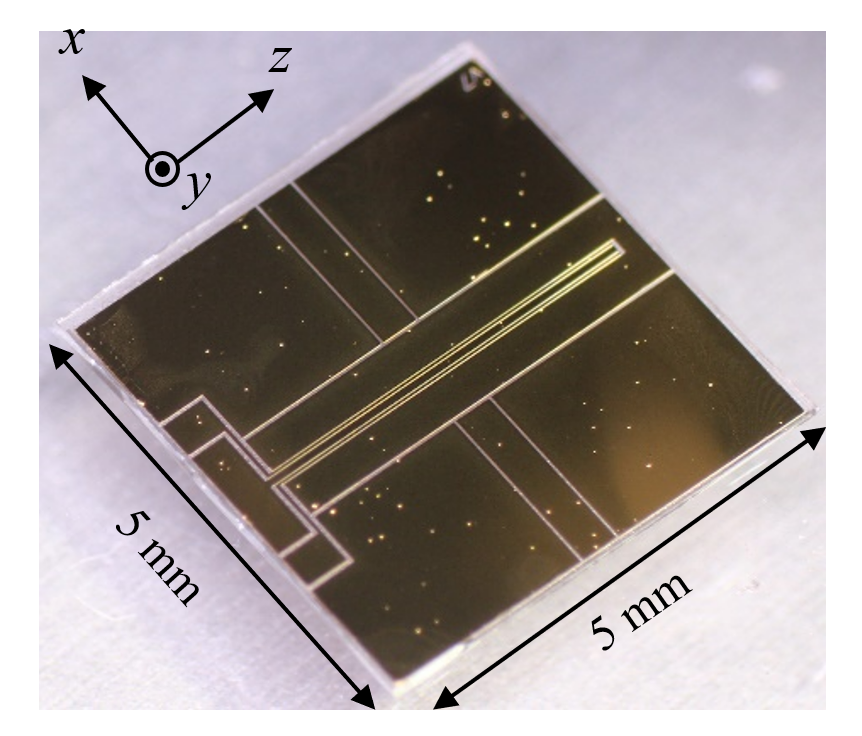
\includegraphics[width = 0.4\linewidth]{./experimental_setup/figure/Using_PlannerTrap.png}
		\caption{本実験で使用するプレーナートラップ}
		\label{fig:PlanarTrap}
	\end{center}
\end{figure}

\section{光学系}
\Fig{optical_system}にイオン捕獲のためのレーザーの光学系を示す.
\begin{figure}[h]
	\centering
		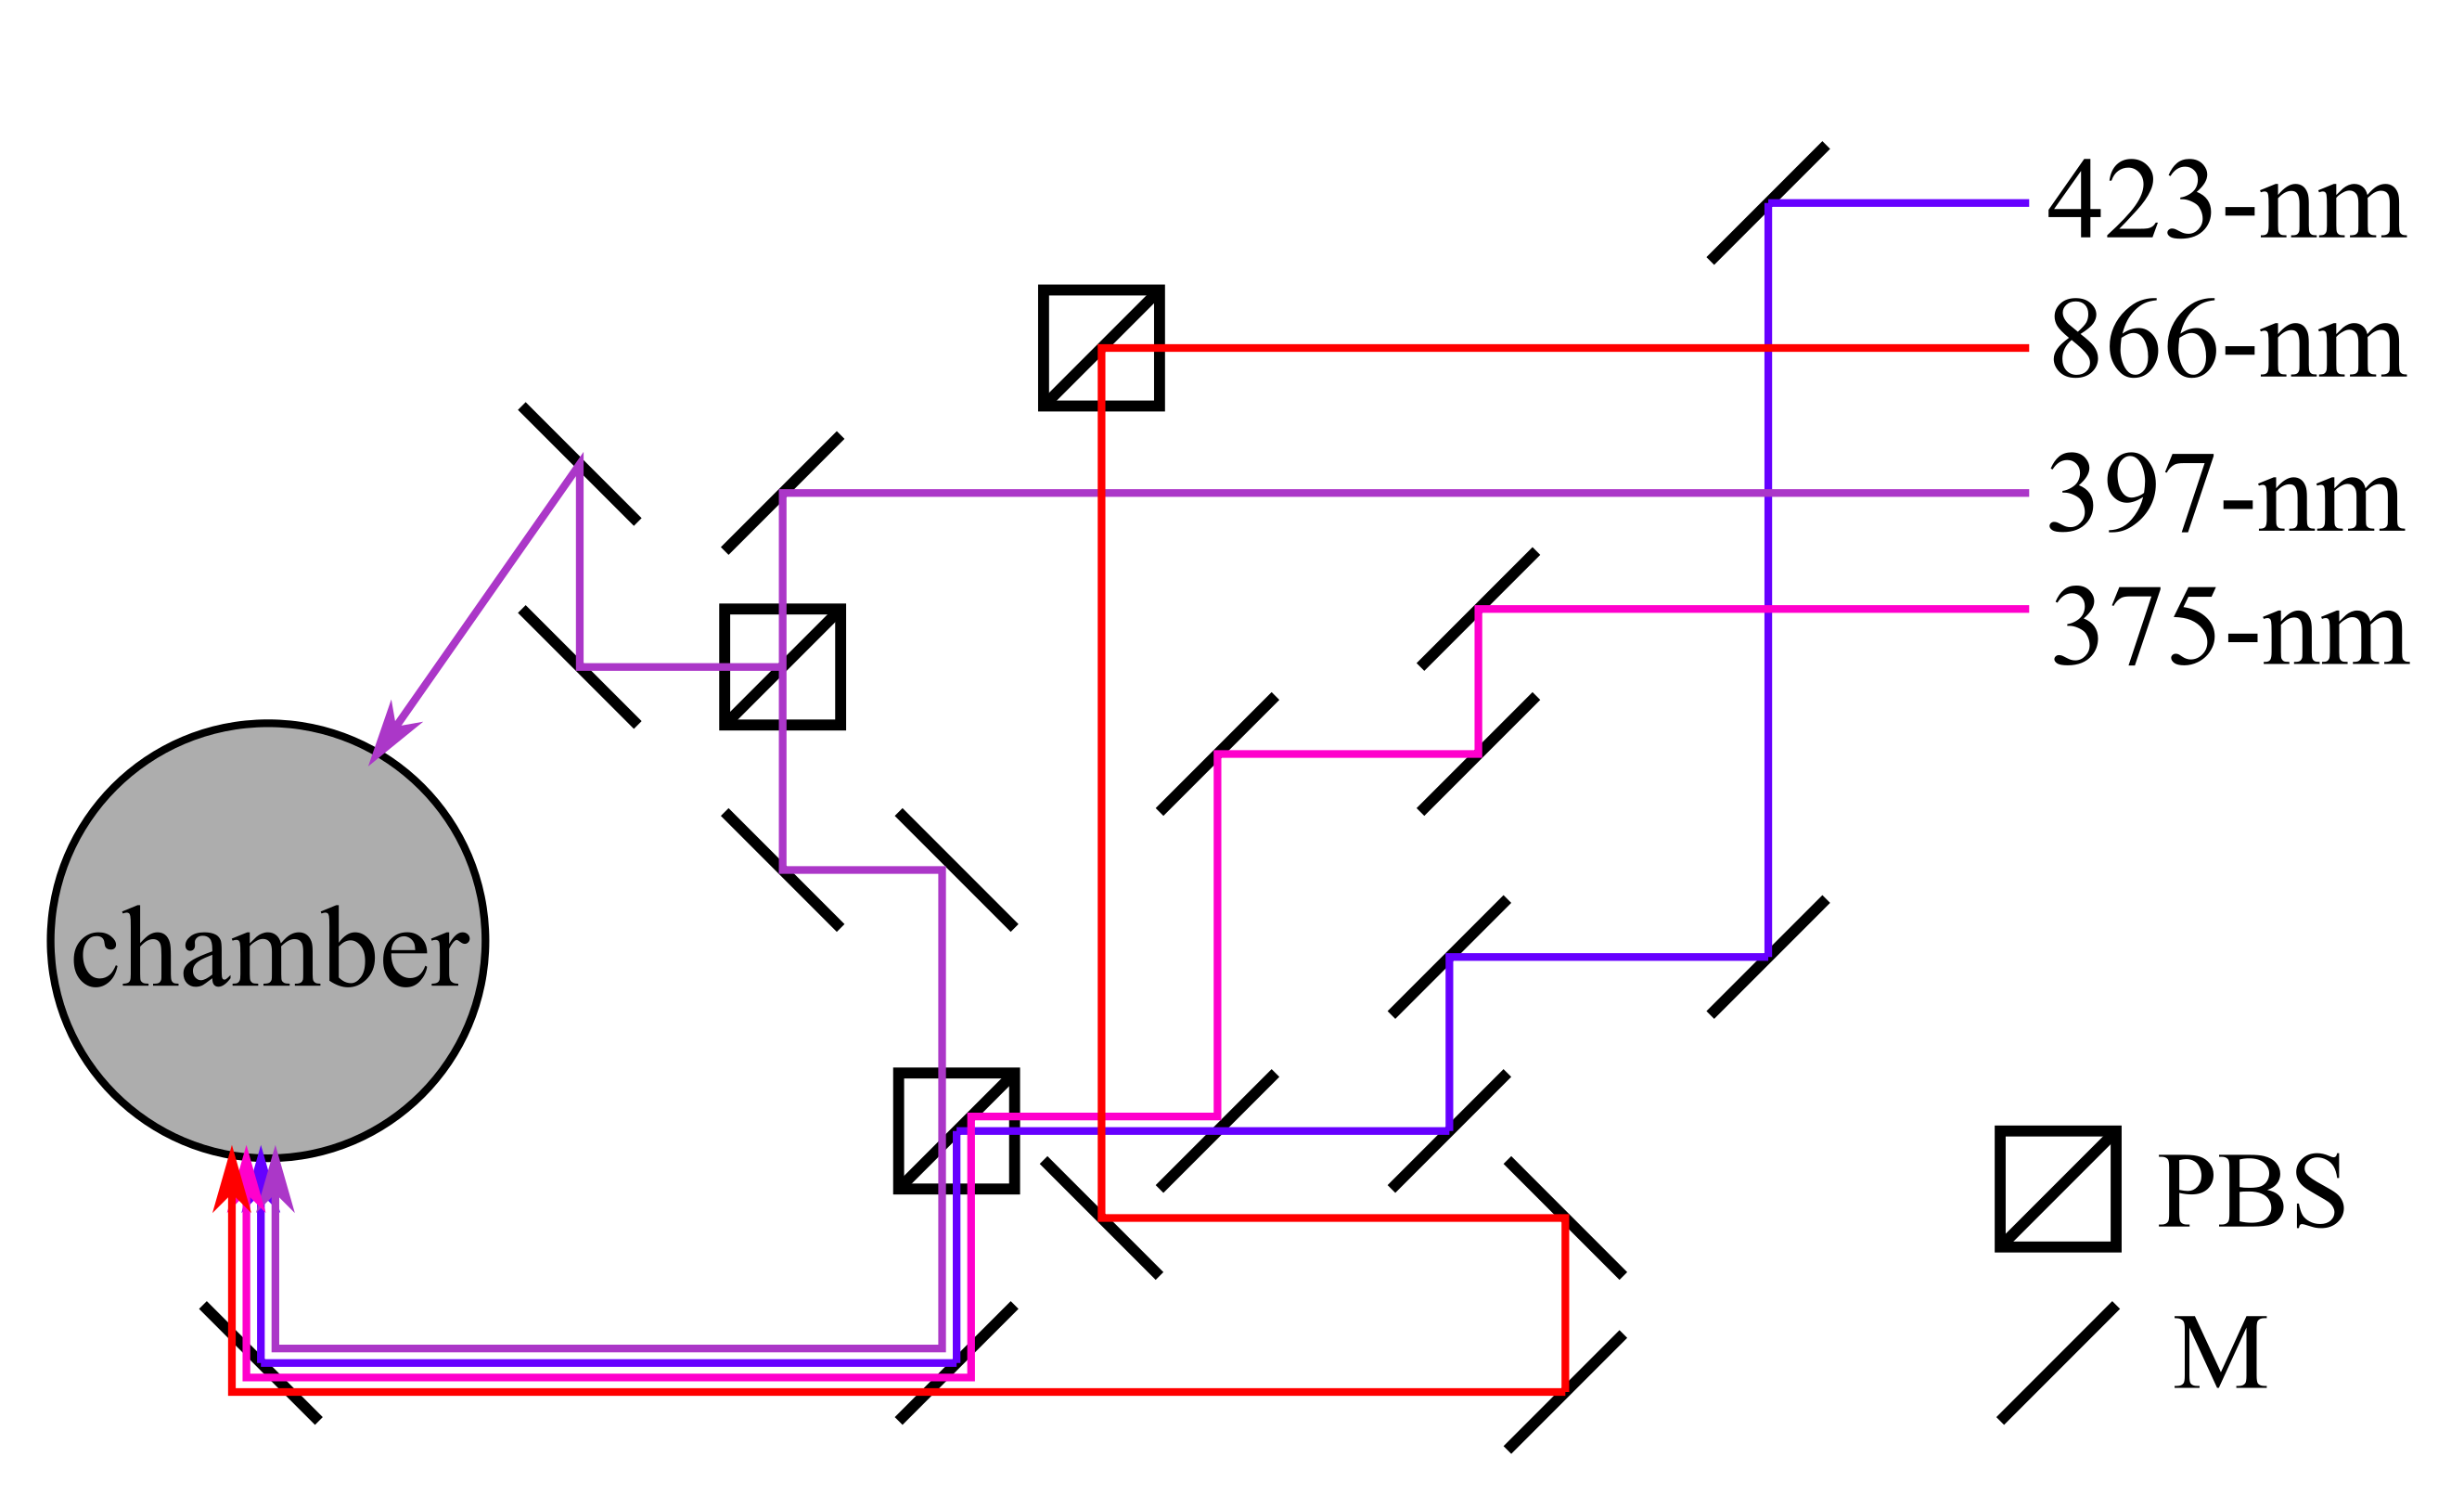
\includegraphics[width = 0.5\linewidth]{./experimental_setup/figure/Optical_System.png}
		\caption{プレーナートラップに照射するレーザーの光学系(M:ミラー,PBS:偏向ビームスプリッター)}
		\label{fig:optical_system}
\end{figure}

\section{レーザー}
\begin{table}[h]
	\centering
		\caption{$^{40}{\rm Ca}^+$を捕獲するときに使用するレーザーの波長}
		\label{tb:use_laser}
			\begin{tabular}{c|c} \hline \hline
				波長系の校正 & 632 nm \\ 
				$^{40}{\rm Ca}$の光イオン化 & 423 nm, 375 nm \\
				$^{40}{\rm Ca}^+$の冷却 & 397 nm \\
				$^{40}{\rm Ca}^+$のリポンプ & 866 nm \\ \hline 
			\end{tabular}
\end{table}
イオントラップに使用するレーザーのビーム径とその強度をスリット走査型光ビームプロファイラ(THORLABS,BP209-VIS/M)とデジタルパワー\&エネルギーメータ(THORLABS,PM100D)およびフォトダイオードパワーセンサー(THORLABS,S120C)を用いて計測を行った.
まず,各レーザーの強度を\Tb{AllLaserPower}に示す.

\begin{table}[h]
	\begin{center}
		\caption{各レーザーのパワー一覧表}
		\label{tab:AllLaserPower}
		\begin{tabular}{c|c} \hline \hline
			波長 (nm) & 強度 ($\mu$W) \\ \hline
			375 &4.1 \\ \hline
			397 &17.4 \\ \hline
			423 &28.4 \\ \hline
			866 &700 \\ \hline
		\end{tabular}
	\end{center}
\end{table}

次に,ビーム径の計測結果を\Fig{AllLaserBeamProfile}に示す.

\begin{figure}[h]
	\begin{center}
	\begin{minipage}{0.48\linewidth}
		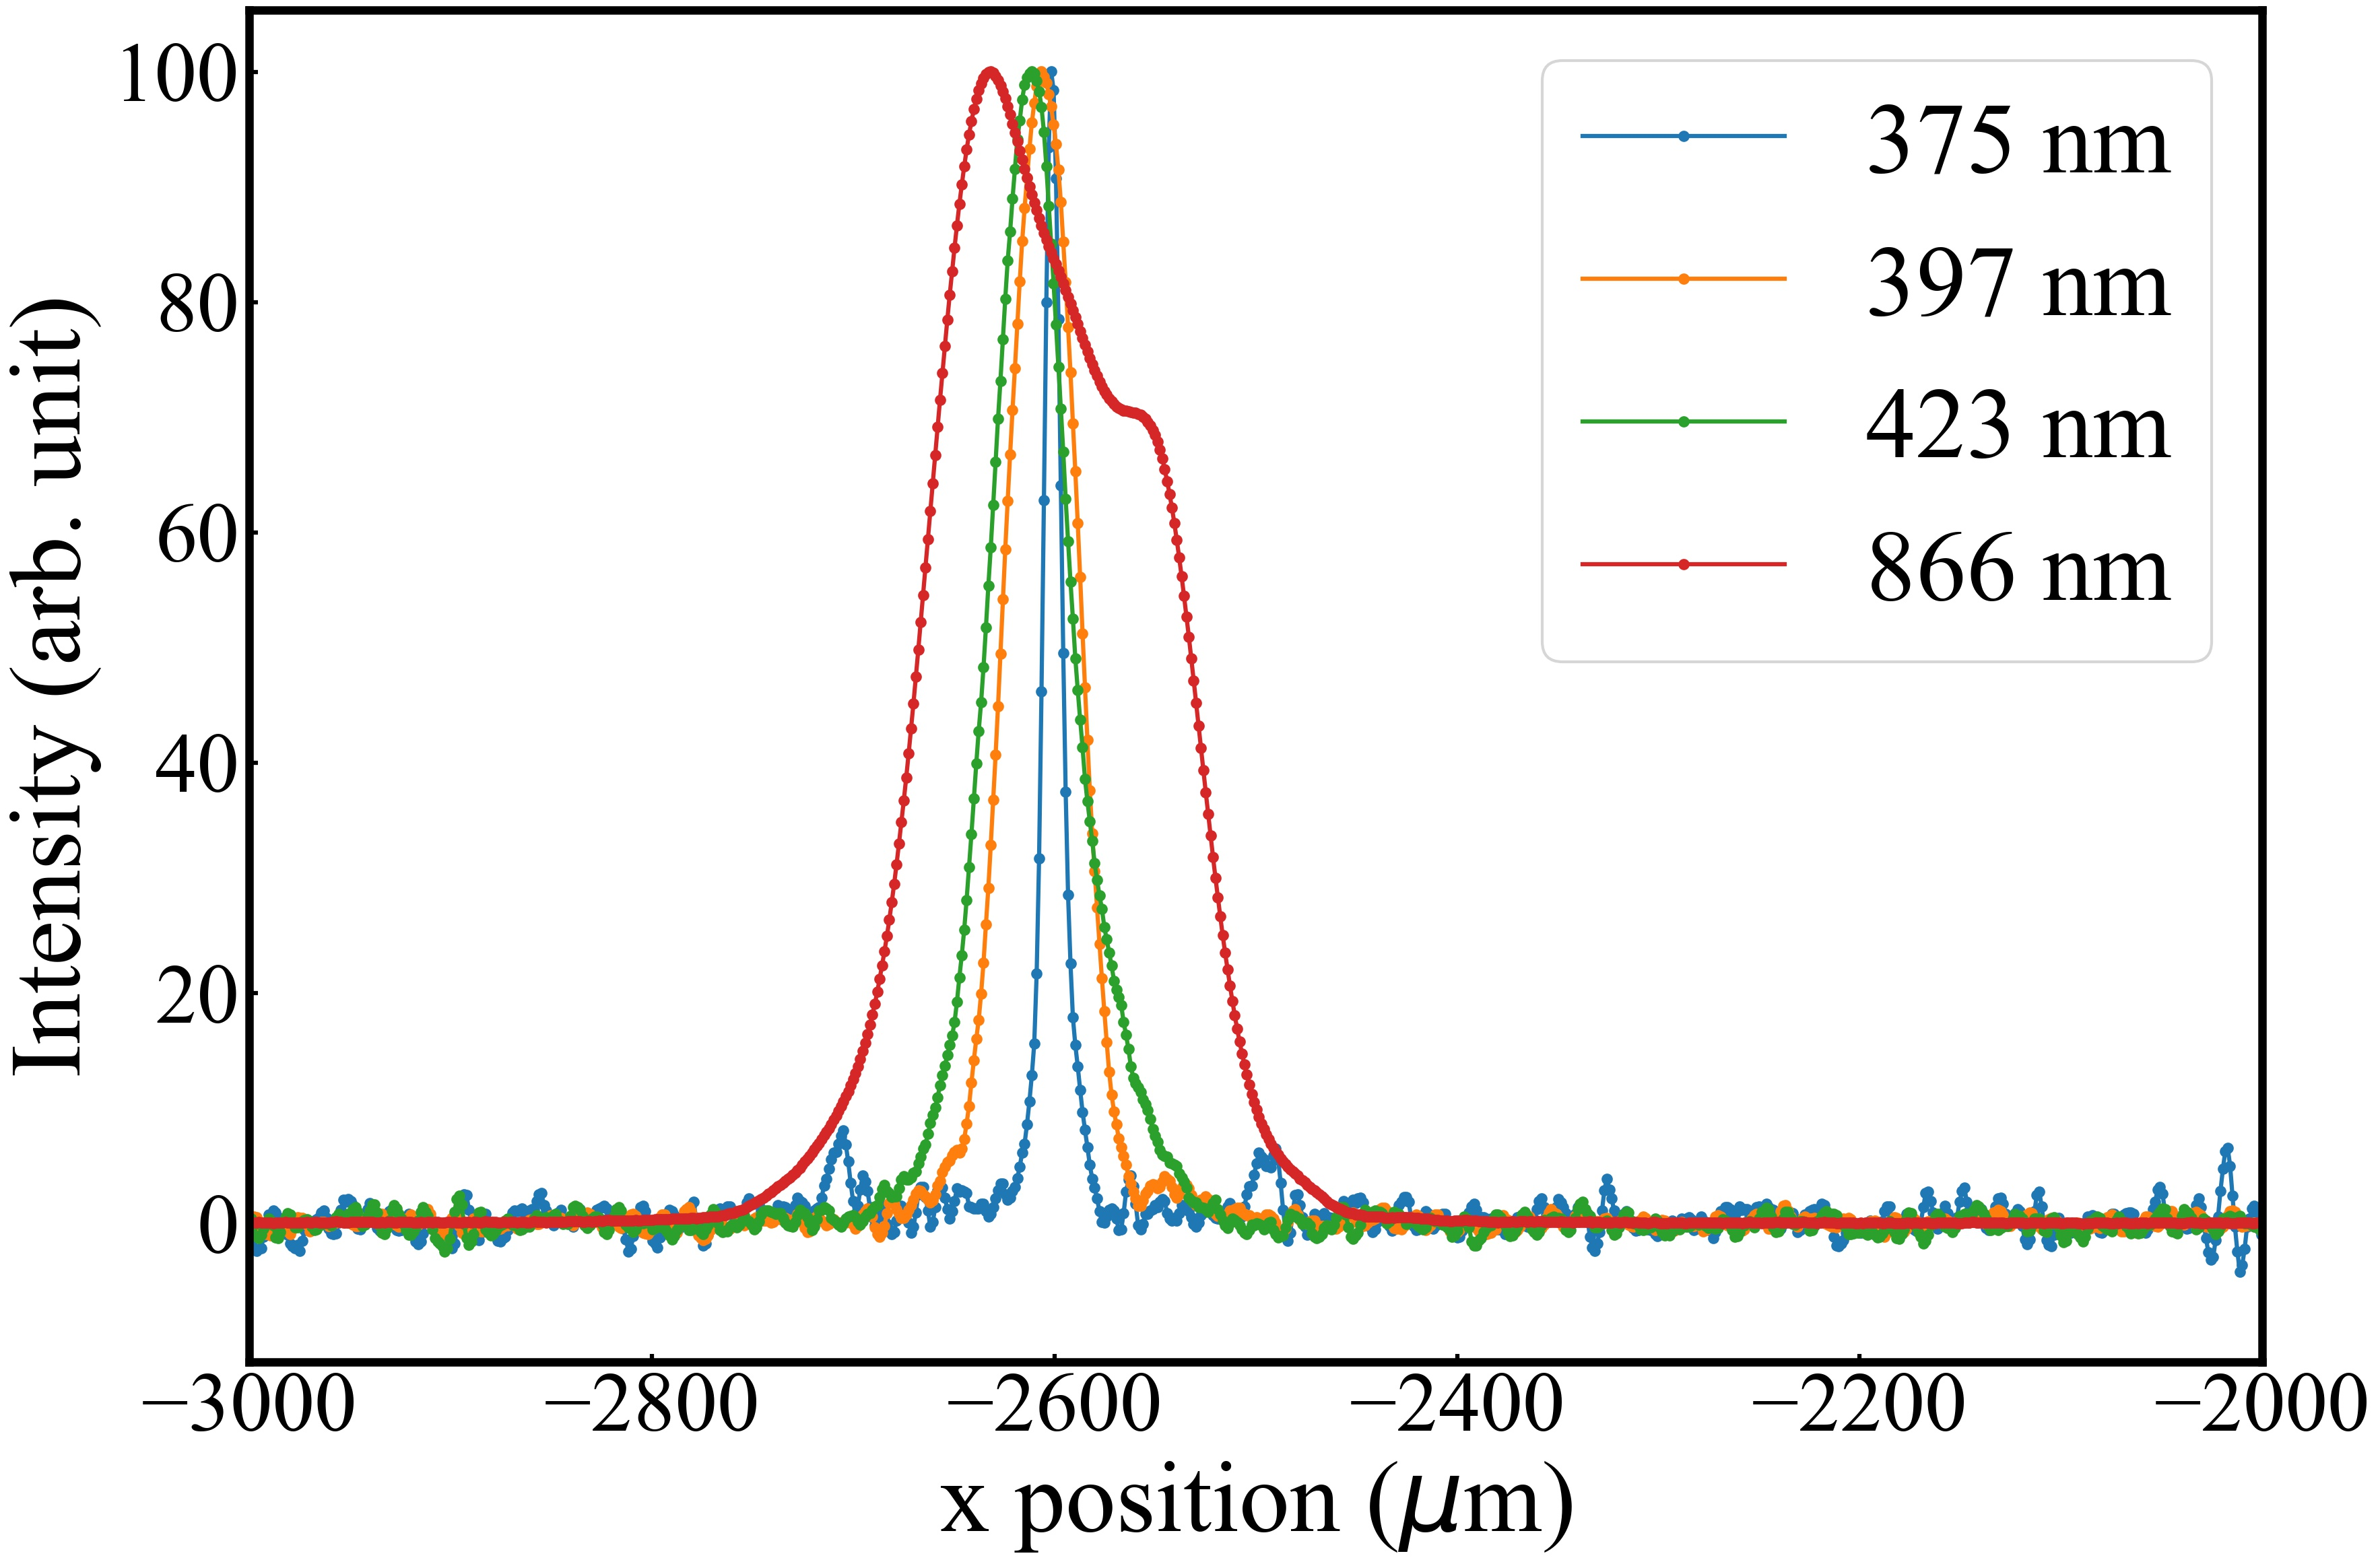
\includegraphics[width = 0.8\columnwidth]{./experimental_setup/figure/AllLaserXpos.jpg}
	\end{minipage}
	\begin{minipage}{0.48\linewidth}
		\begin{center}
		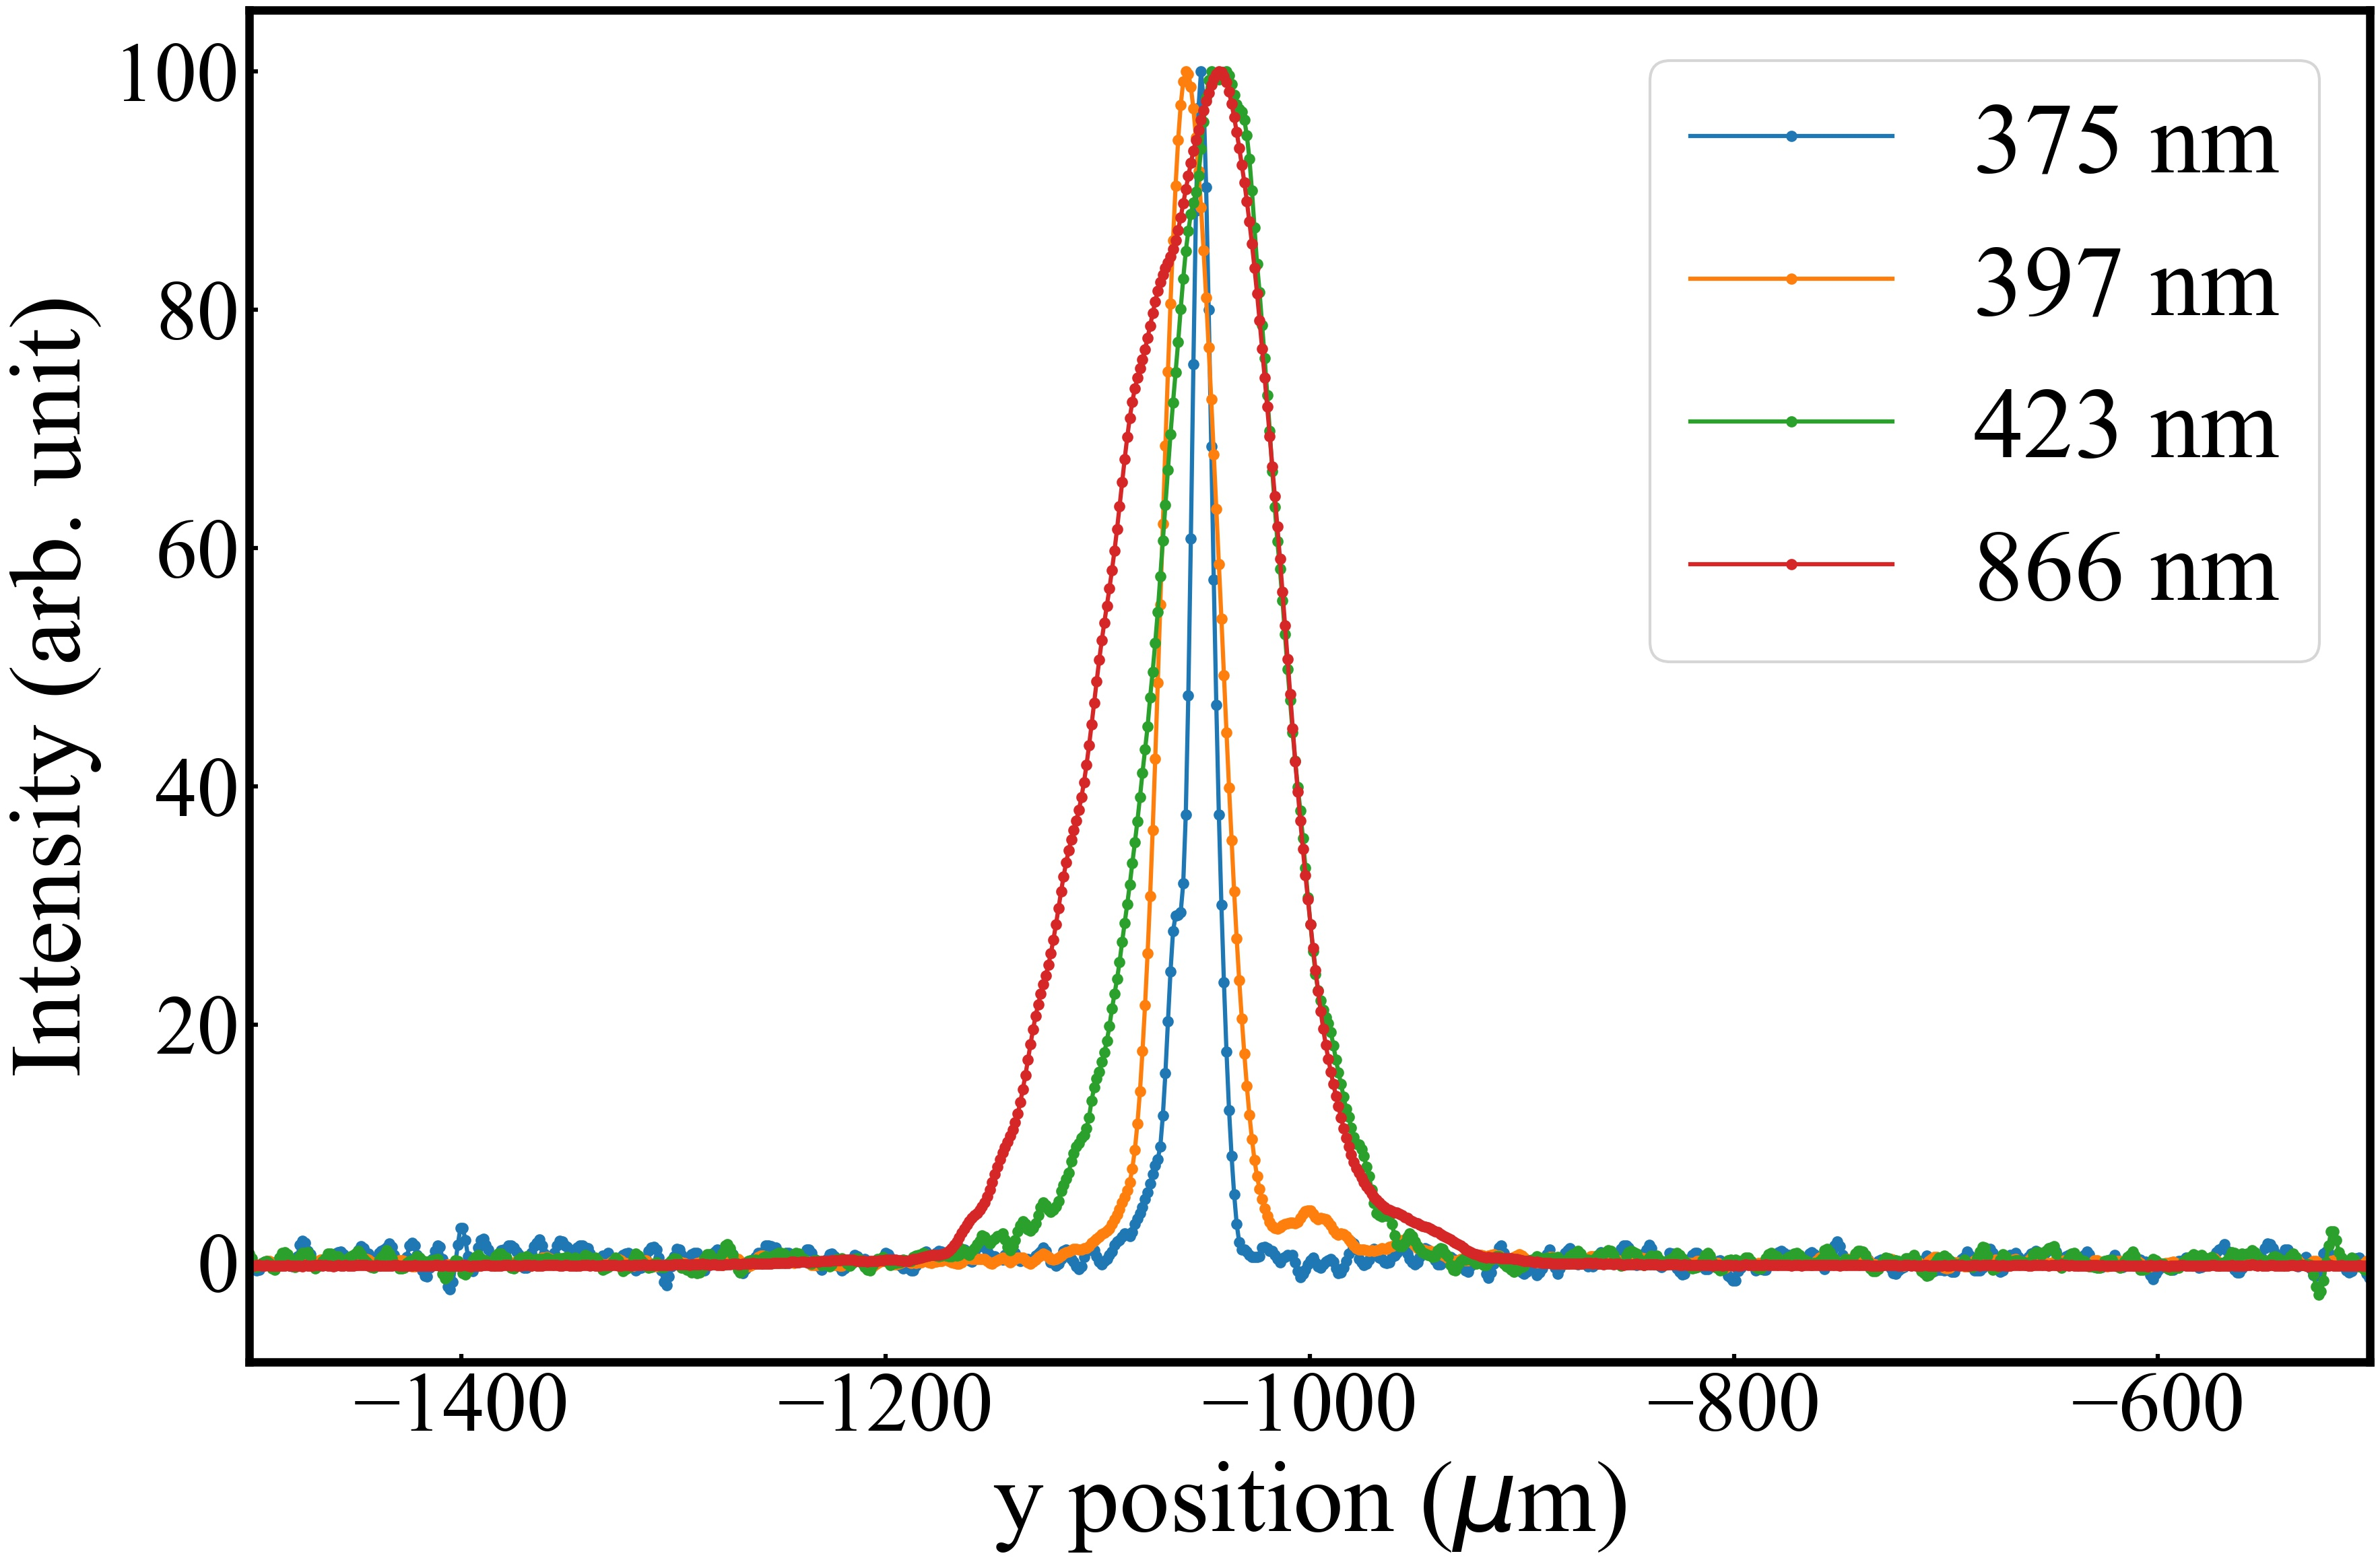
\includegraphics[width = 0.8\columnwidth]{./experimental_setup/figure/AllLaserYpos.jpg}
		\end{center}
	\end{minipage}
	\caption{4種類のレーザーのx,y方向についてのビームプロファイル結果}
	\label{fig:AllLaserBeamProfile}
	\end{center}
\end{figure}

そして,得られたビームプロファイルにガウシアンによるフィッティングを行った様子を\Fig{GaussianFitting}に示し,その結果を\Tb{GaussianFitting}にまとめている.

\begin{table}[h]
	\begin{center}
		\caption{ビームプロファイラで得られた各ビームのプロファイルにガウシアンフィッティングをかけて得られたパラメータ}
		\label{tab:GaussianFitting}
		\begin{tabular}{c|cc|cc} \hline \hline
			波長 (nm)&位置($x$) ($\mu$m)&ビーム径($r_x$) ($\mu$m) &位置($y$) ($\mu$m)& ビーム径($r_y$) ($\mu$m)\\ \hline
			375&-2600.82$\pm$0.03&6.96$\pm$0.05&-1051.14$\pm$0.03&9.37$\pm$0.04 \\
			397&-2606.08$\pm$0.02&24.21$\pm$0.04&-1056.17$\pm$0.02&18.45$\pm$0.02 \\
			423&-2611.55$\pm$0.05&30.20$\pm$0.07&1042.25$\pm$0.03&39.85$\pm$0.05 \\
			866&-2606.1$\pm$0.1&77.2$\pm$0.2&-1054.24$\pm$0.06&54.72$\pm$0.09 \\\hline
		\end{tabular}
	\end{center}
\end{table}

\clearpage

\begin{figure}[h]
	\begin{center}
	%%%12
	\begin{minipage}{0.48\linewidth}
	\begin{center}
			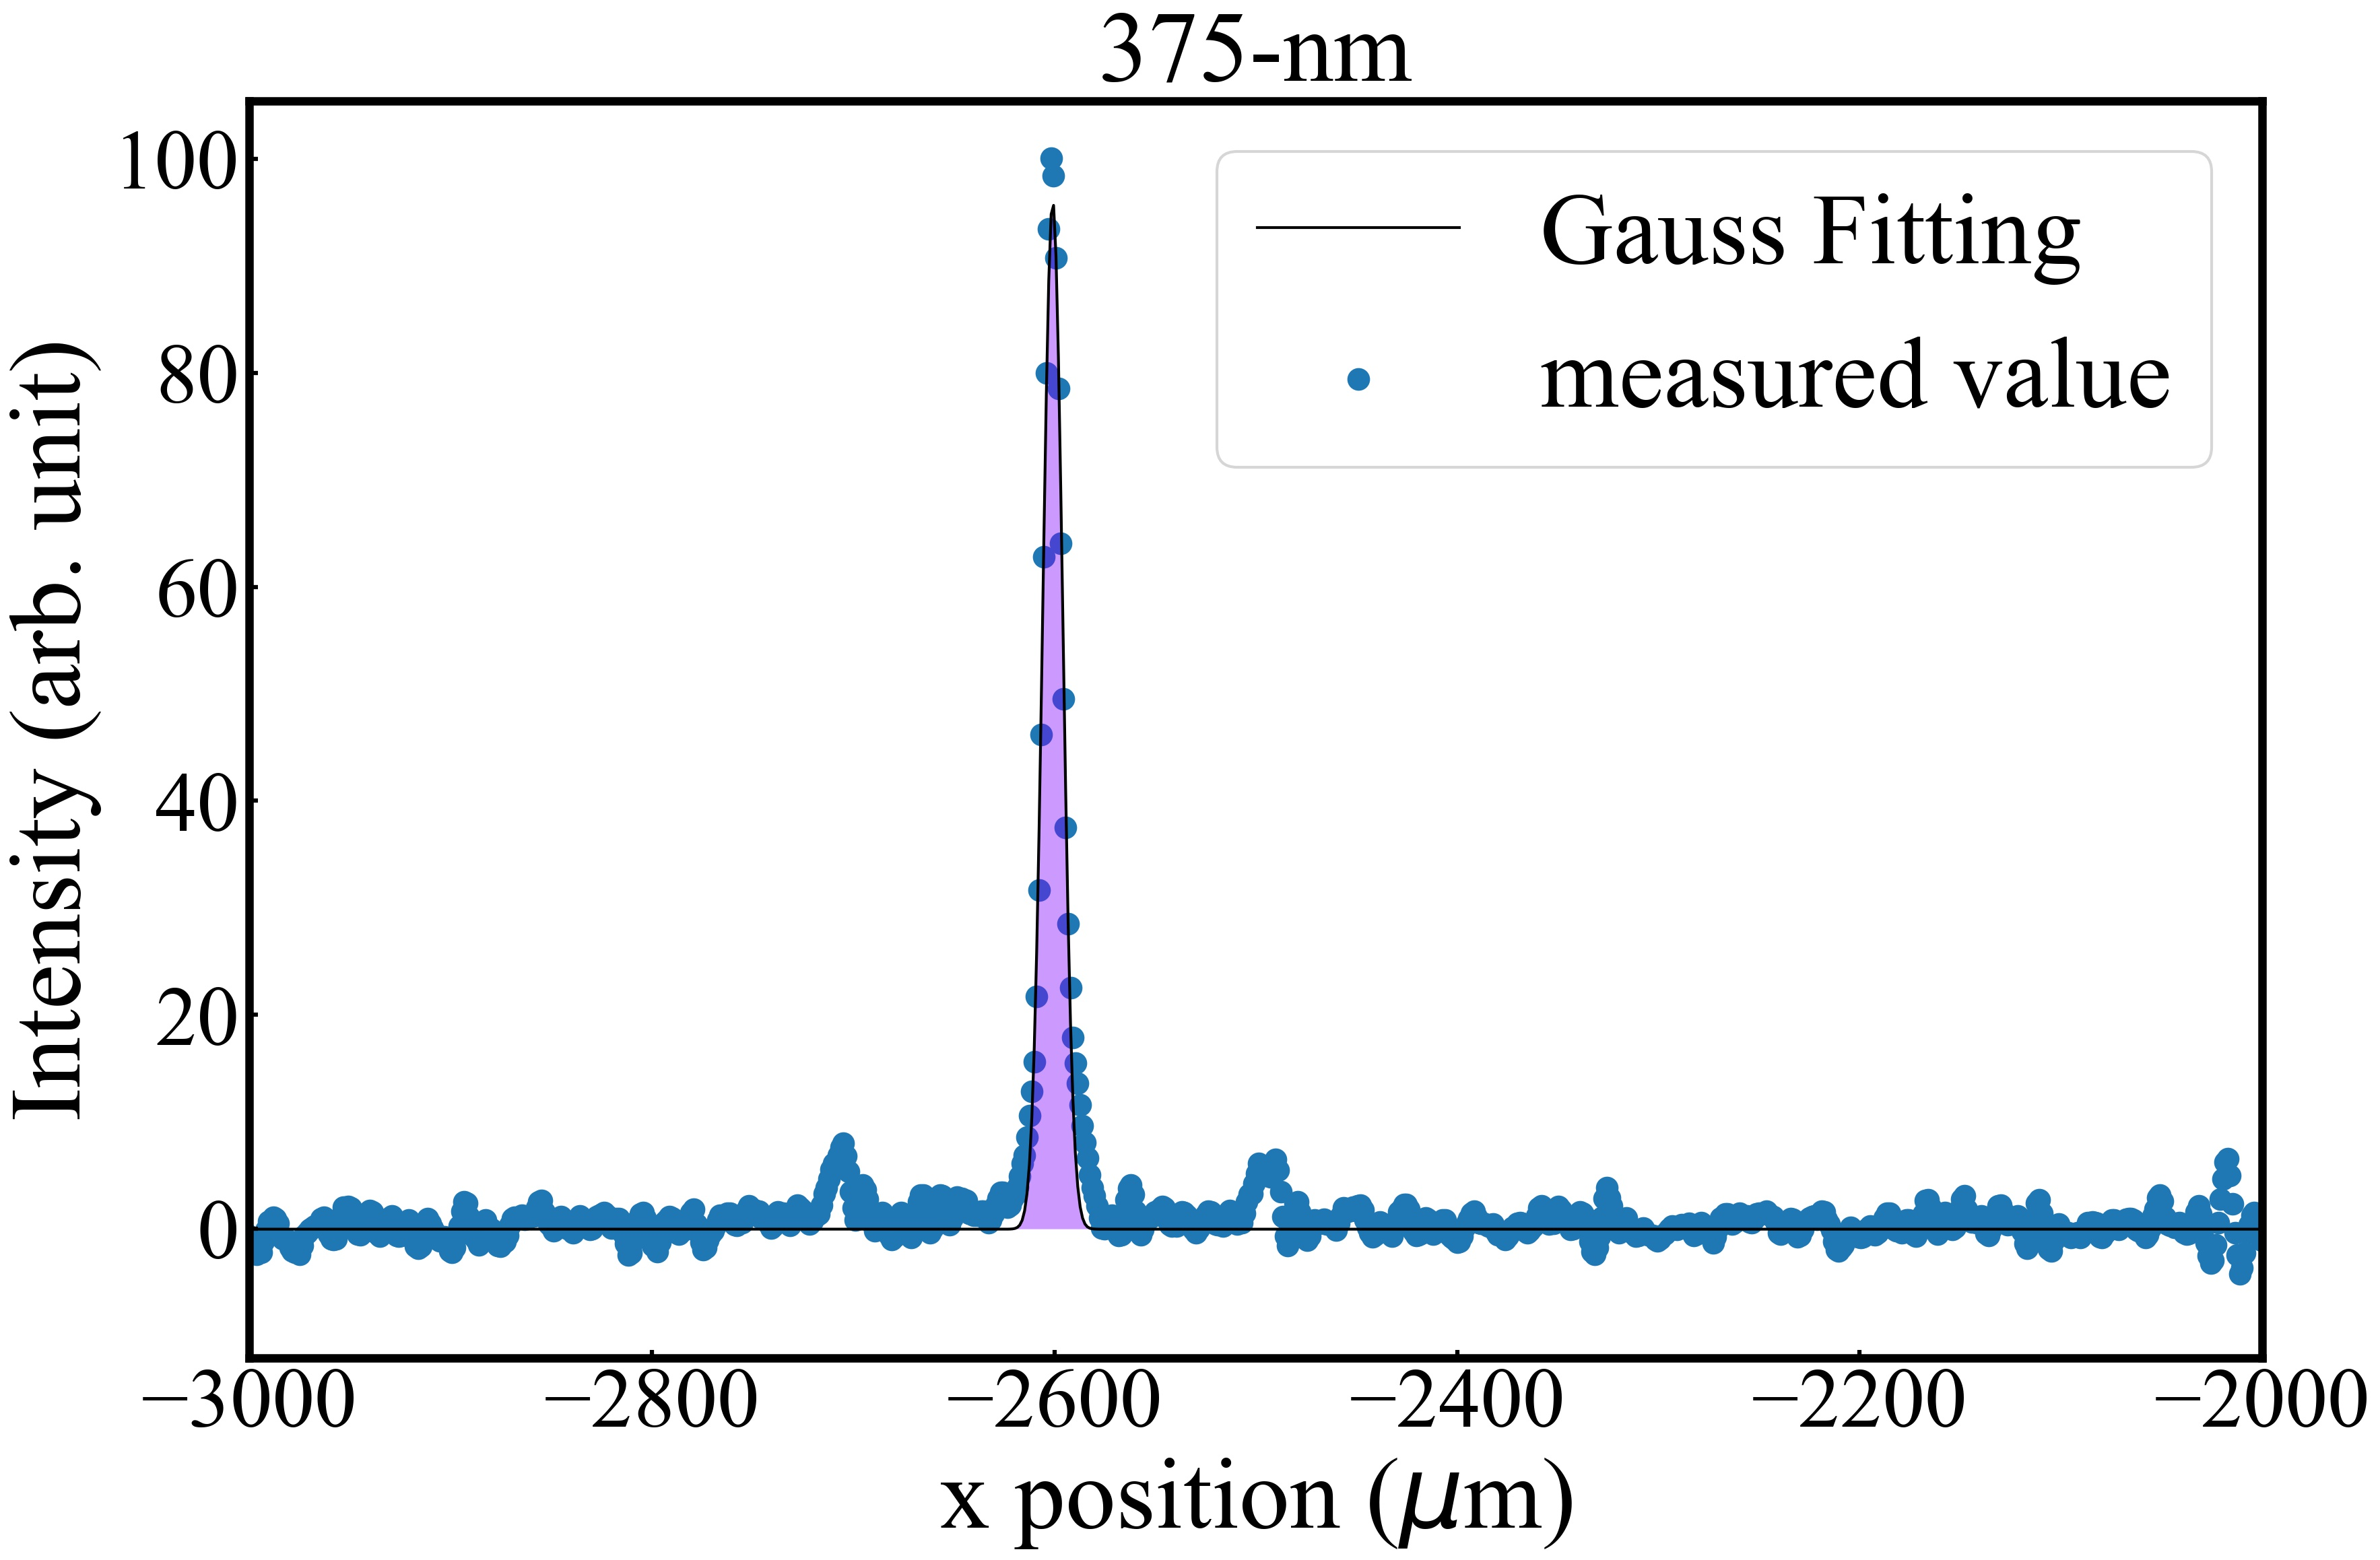
\includegraphics[width = 0.98\columnwidth]{./experimental_setup/figure/375GaussianFittingXpos.jpg}
	\end{center}
	\end{minipage}
	\begin{minipage}{0.48\linewidth}
	\begin{center}
			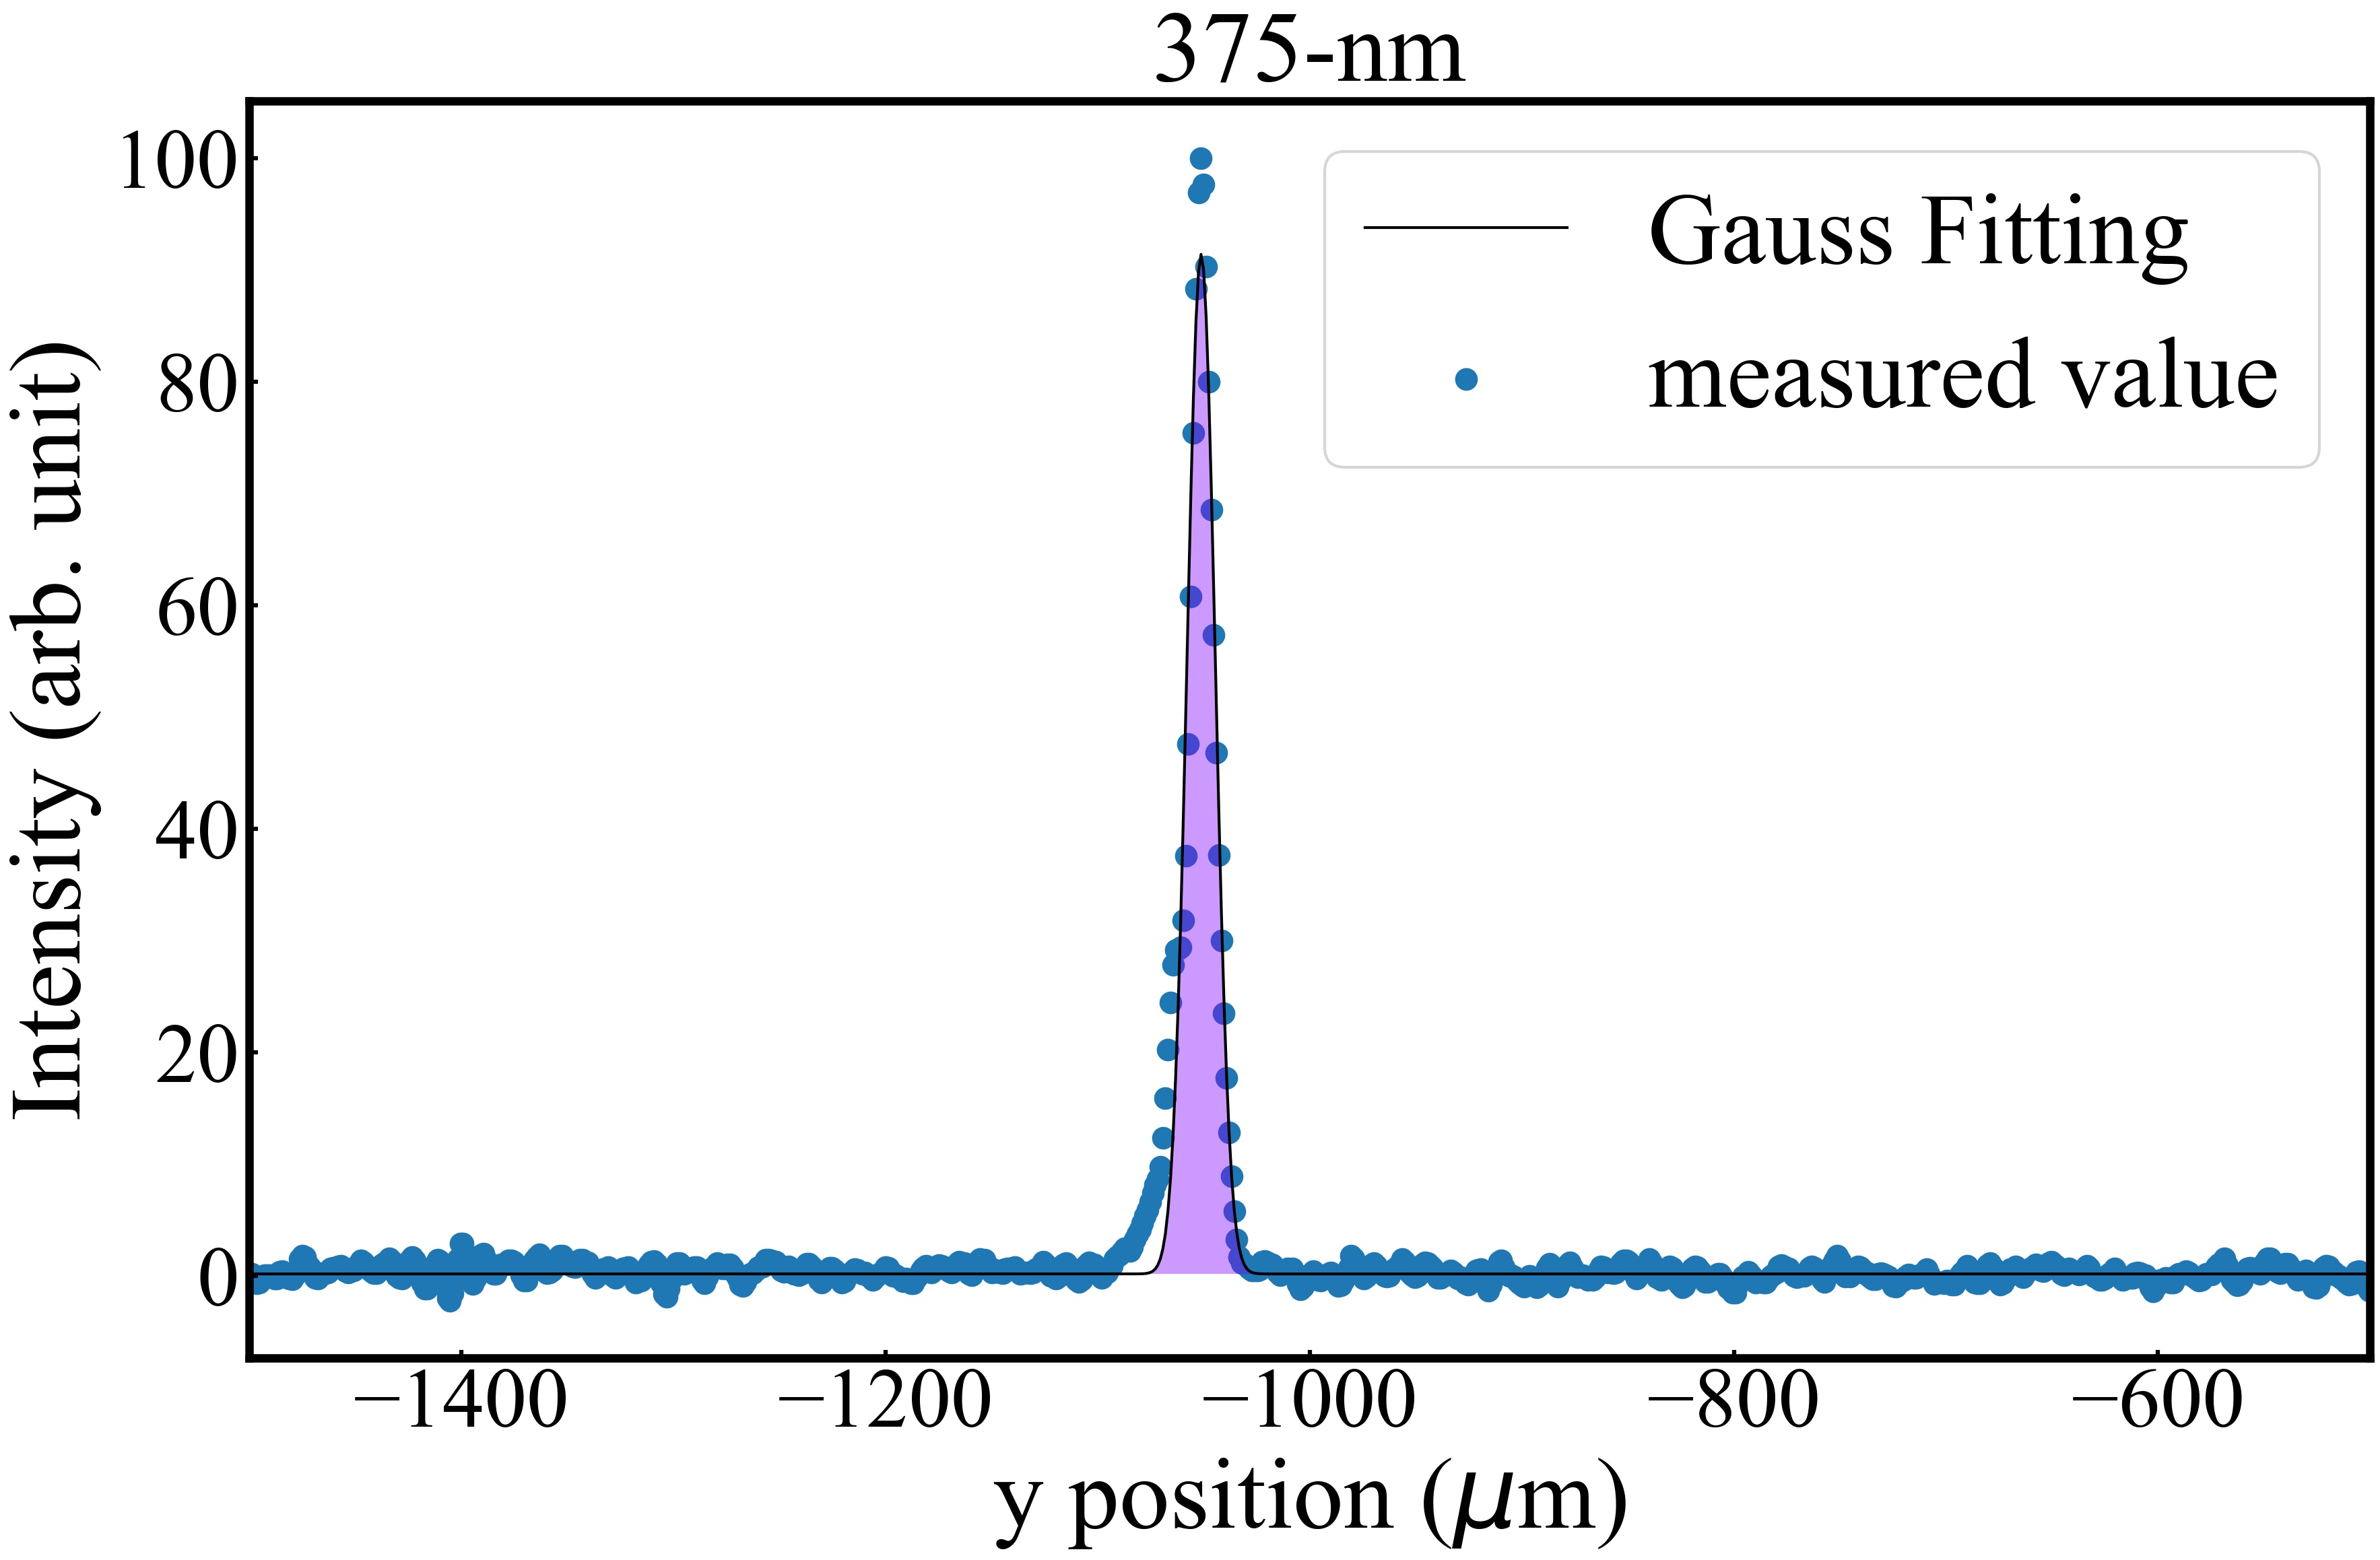
\includegraphics[width=0.98\columnwidth]{./experimental_setup/figure/375GaussianFittingYpos.jpg}
	\end{center}
	\end{minipage}
	%%%34
	\begin{minipage}{0.48\linewidth}
	\begin{center}
		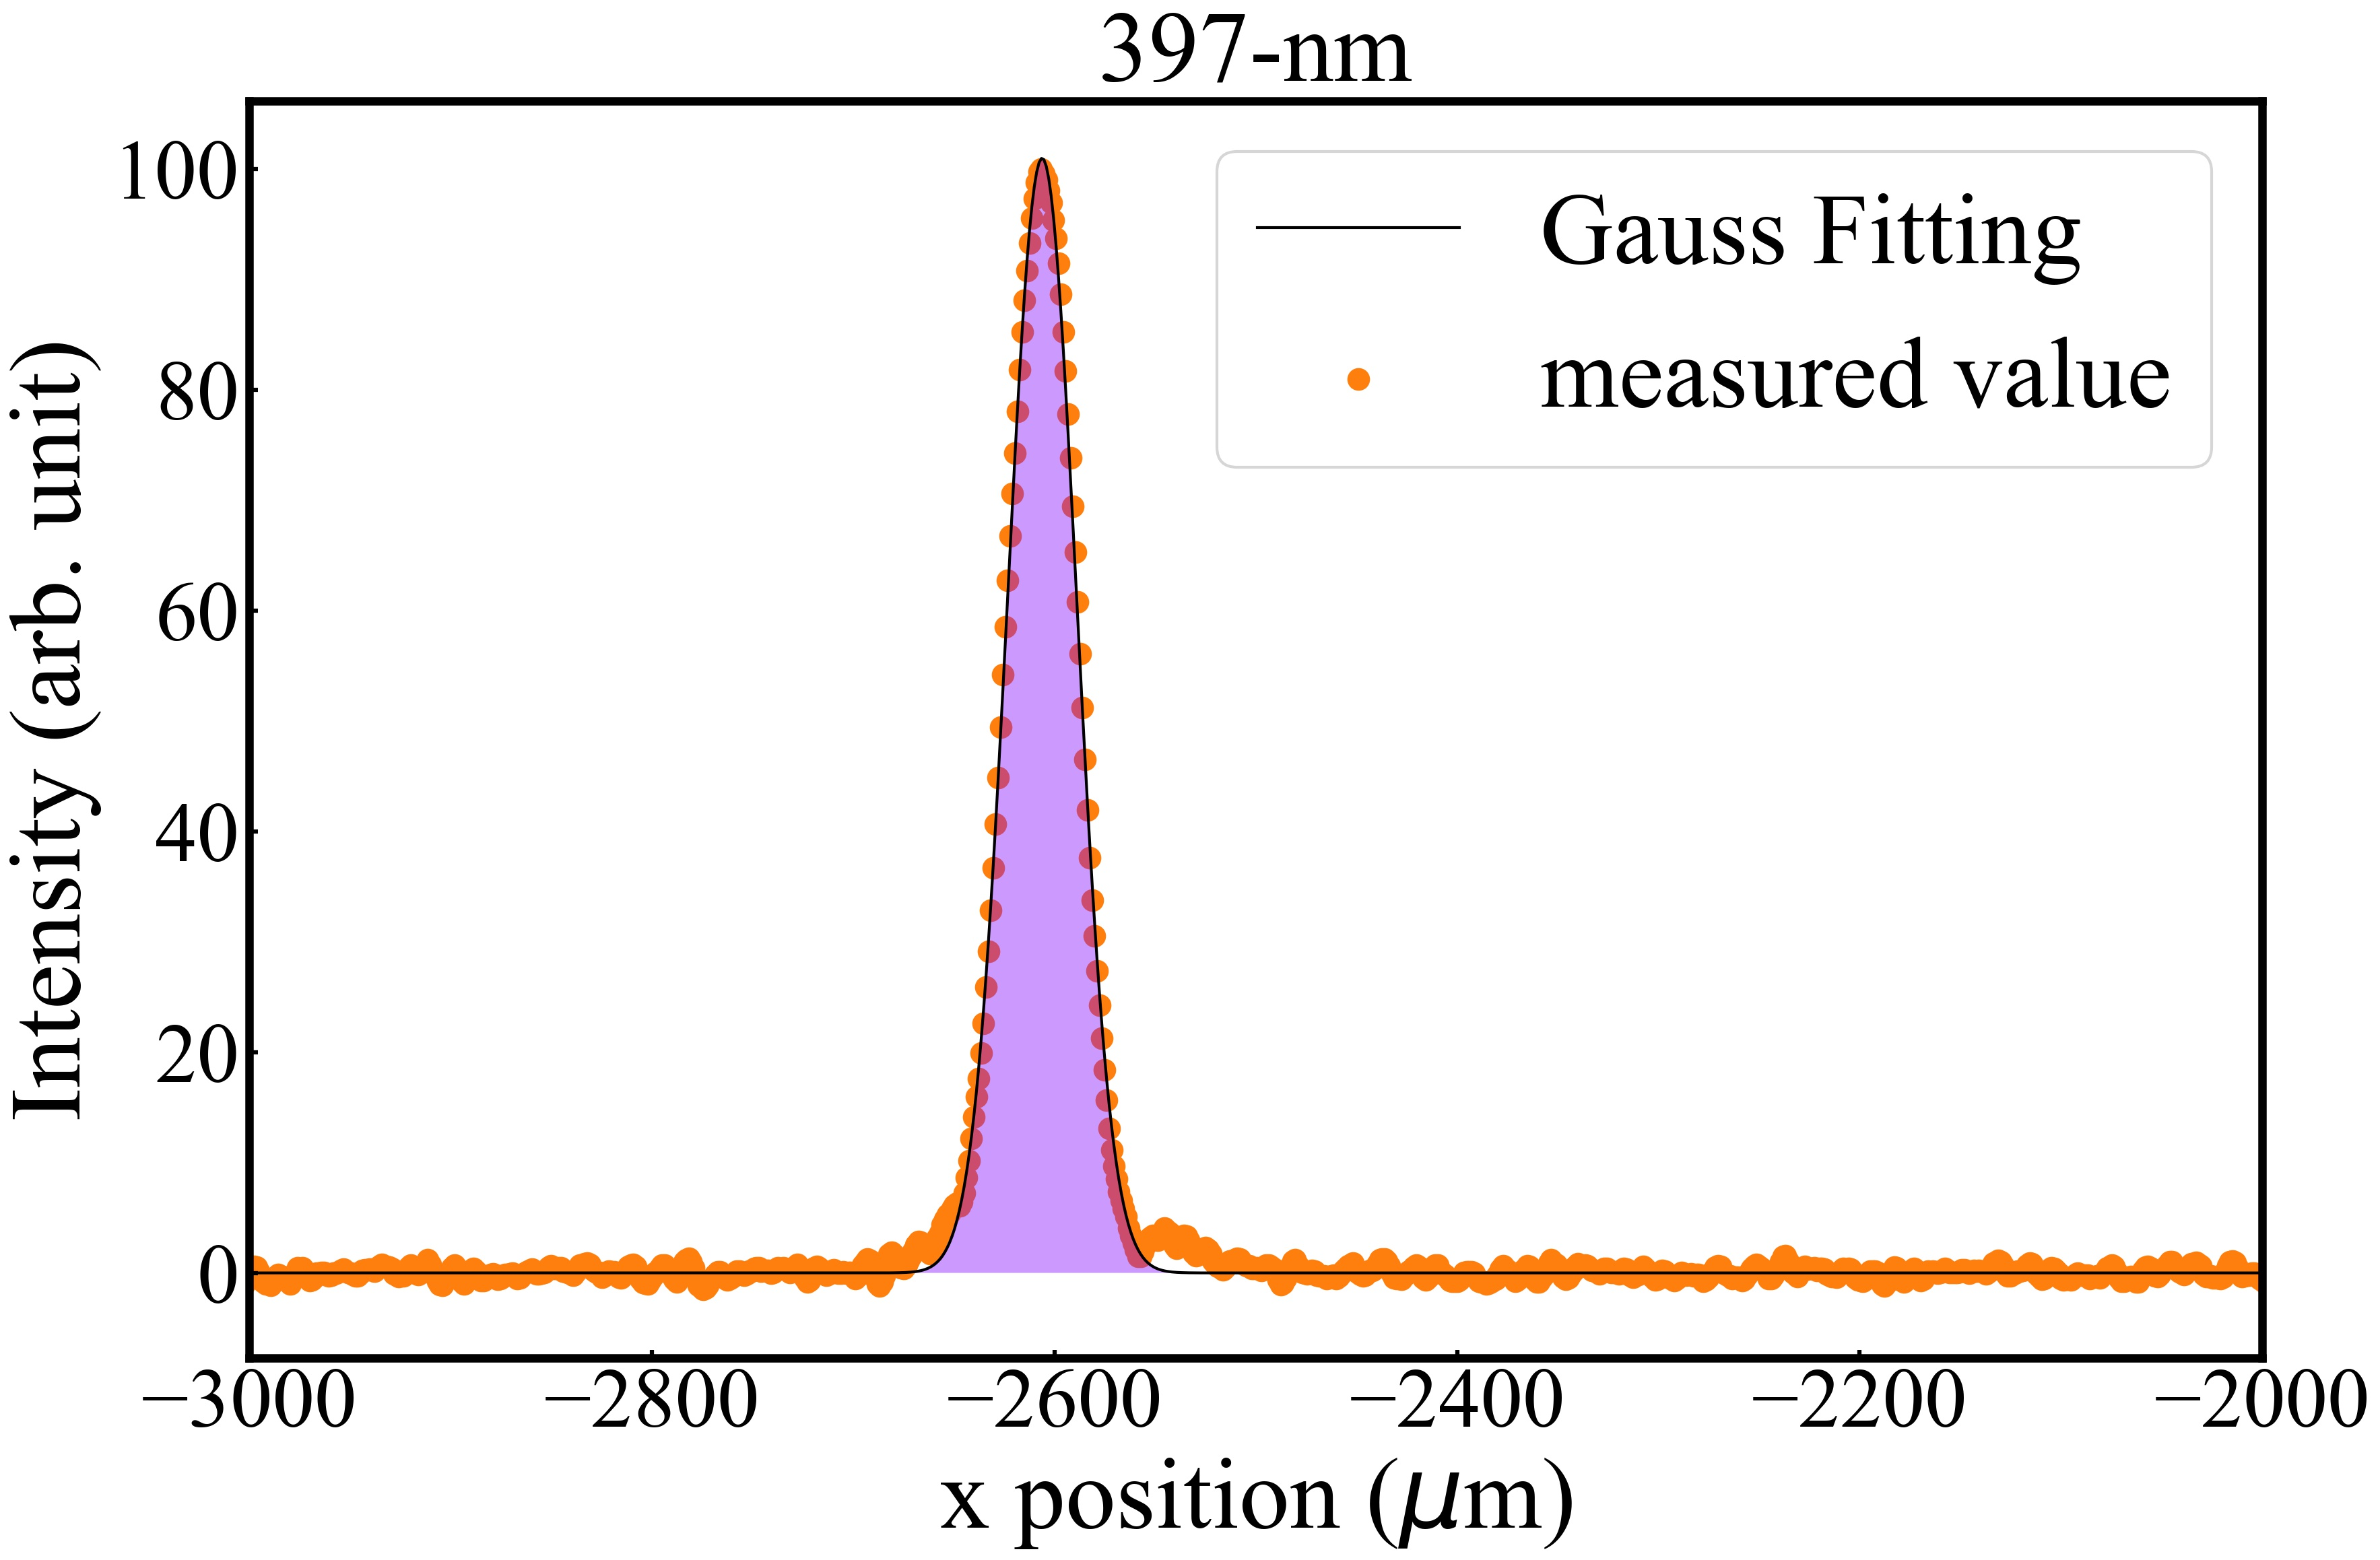
\includegraphics[width = 0.98\columnwidth]{./experimental_setup/figure/397GaussianFittingXpos.jpg}
	\end{center}
	\end{minipage}
	\begin{minipage}{0.48\linewidth}
	\begin{center}
		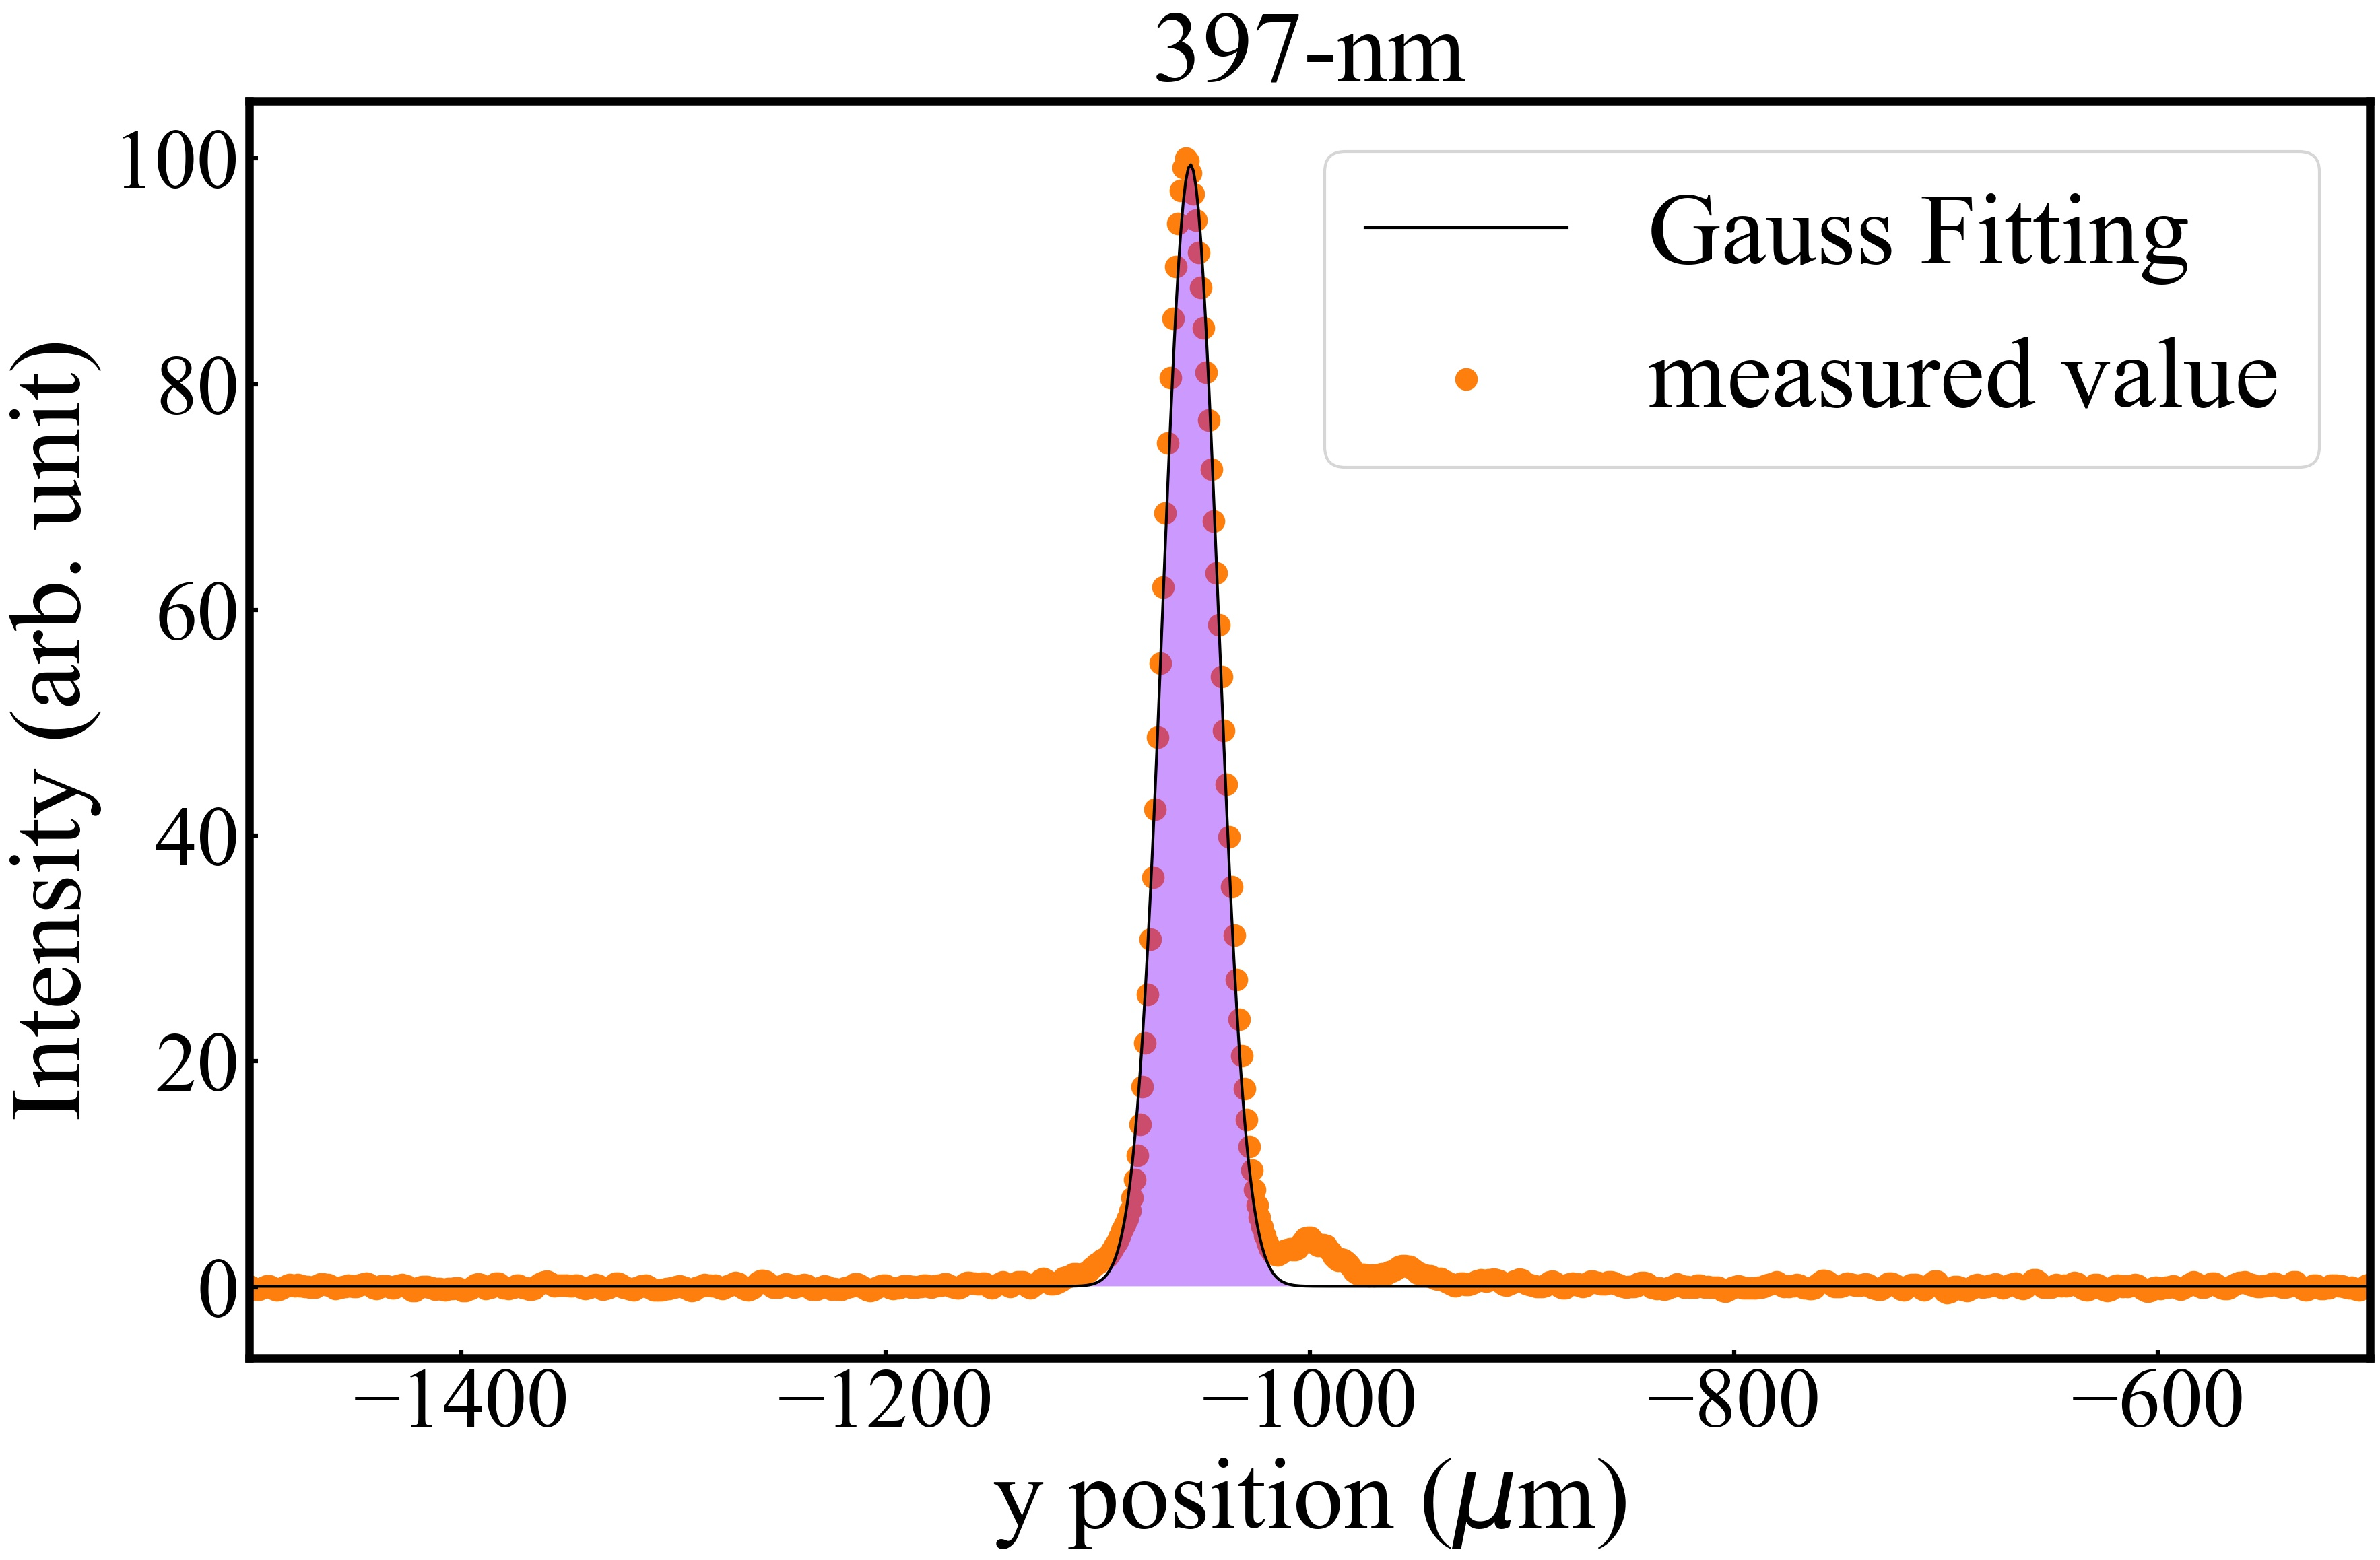
\includegraphics[width=0.98\columnwidth]{./experimental_setup/figure/397GaussianFittingYpos.jpg}
	\end{center}
	\end{minipage}
	%%%56
	\begin{minipage}{0.48\linewidth}
	\begin{center}
		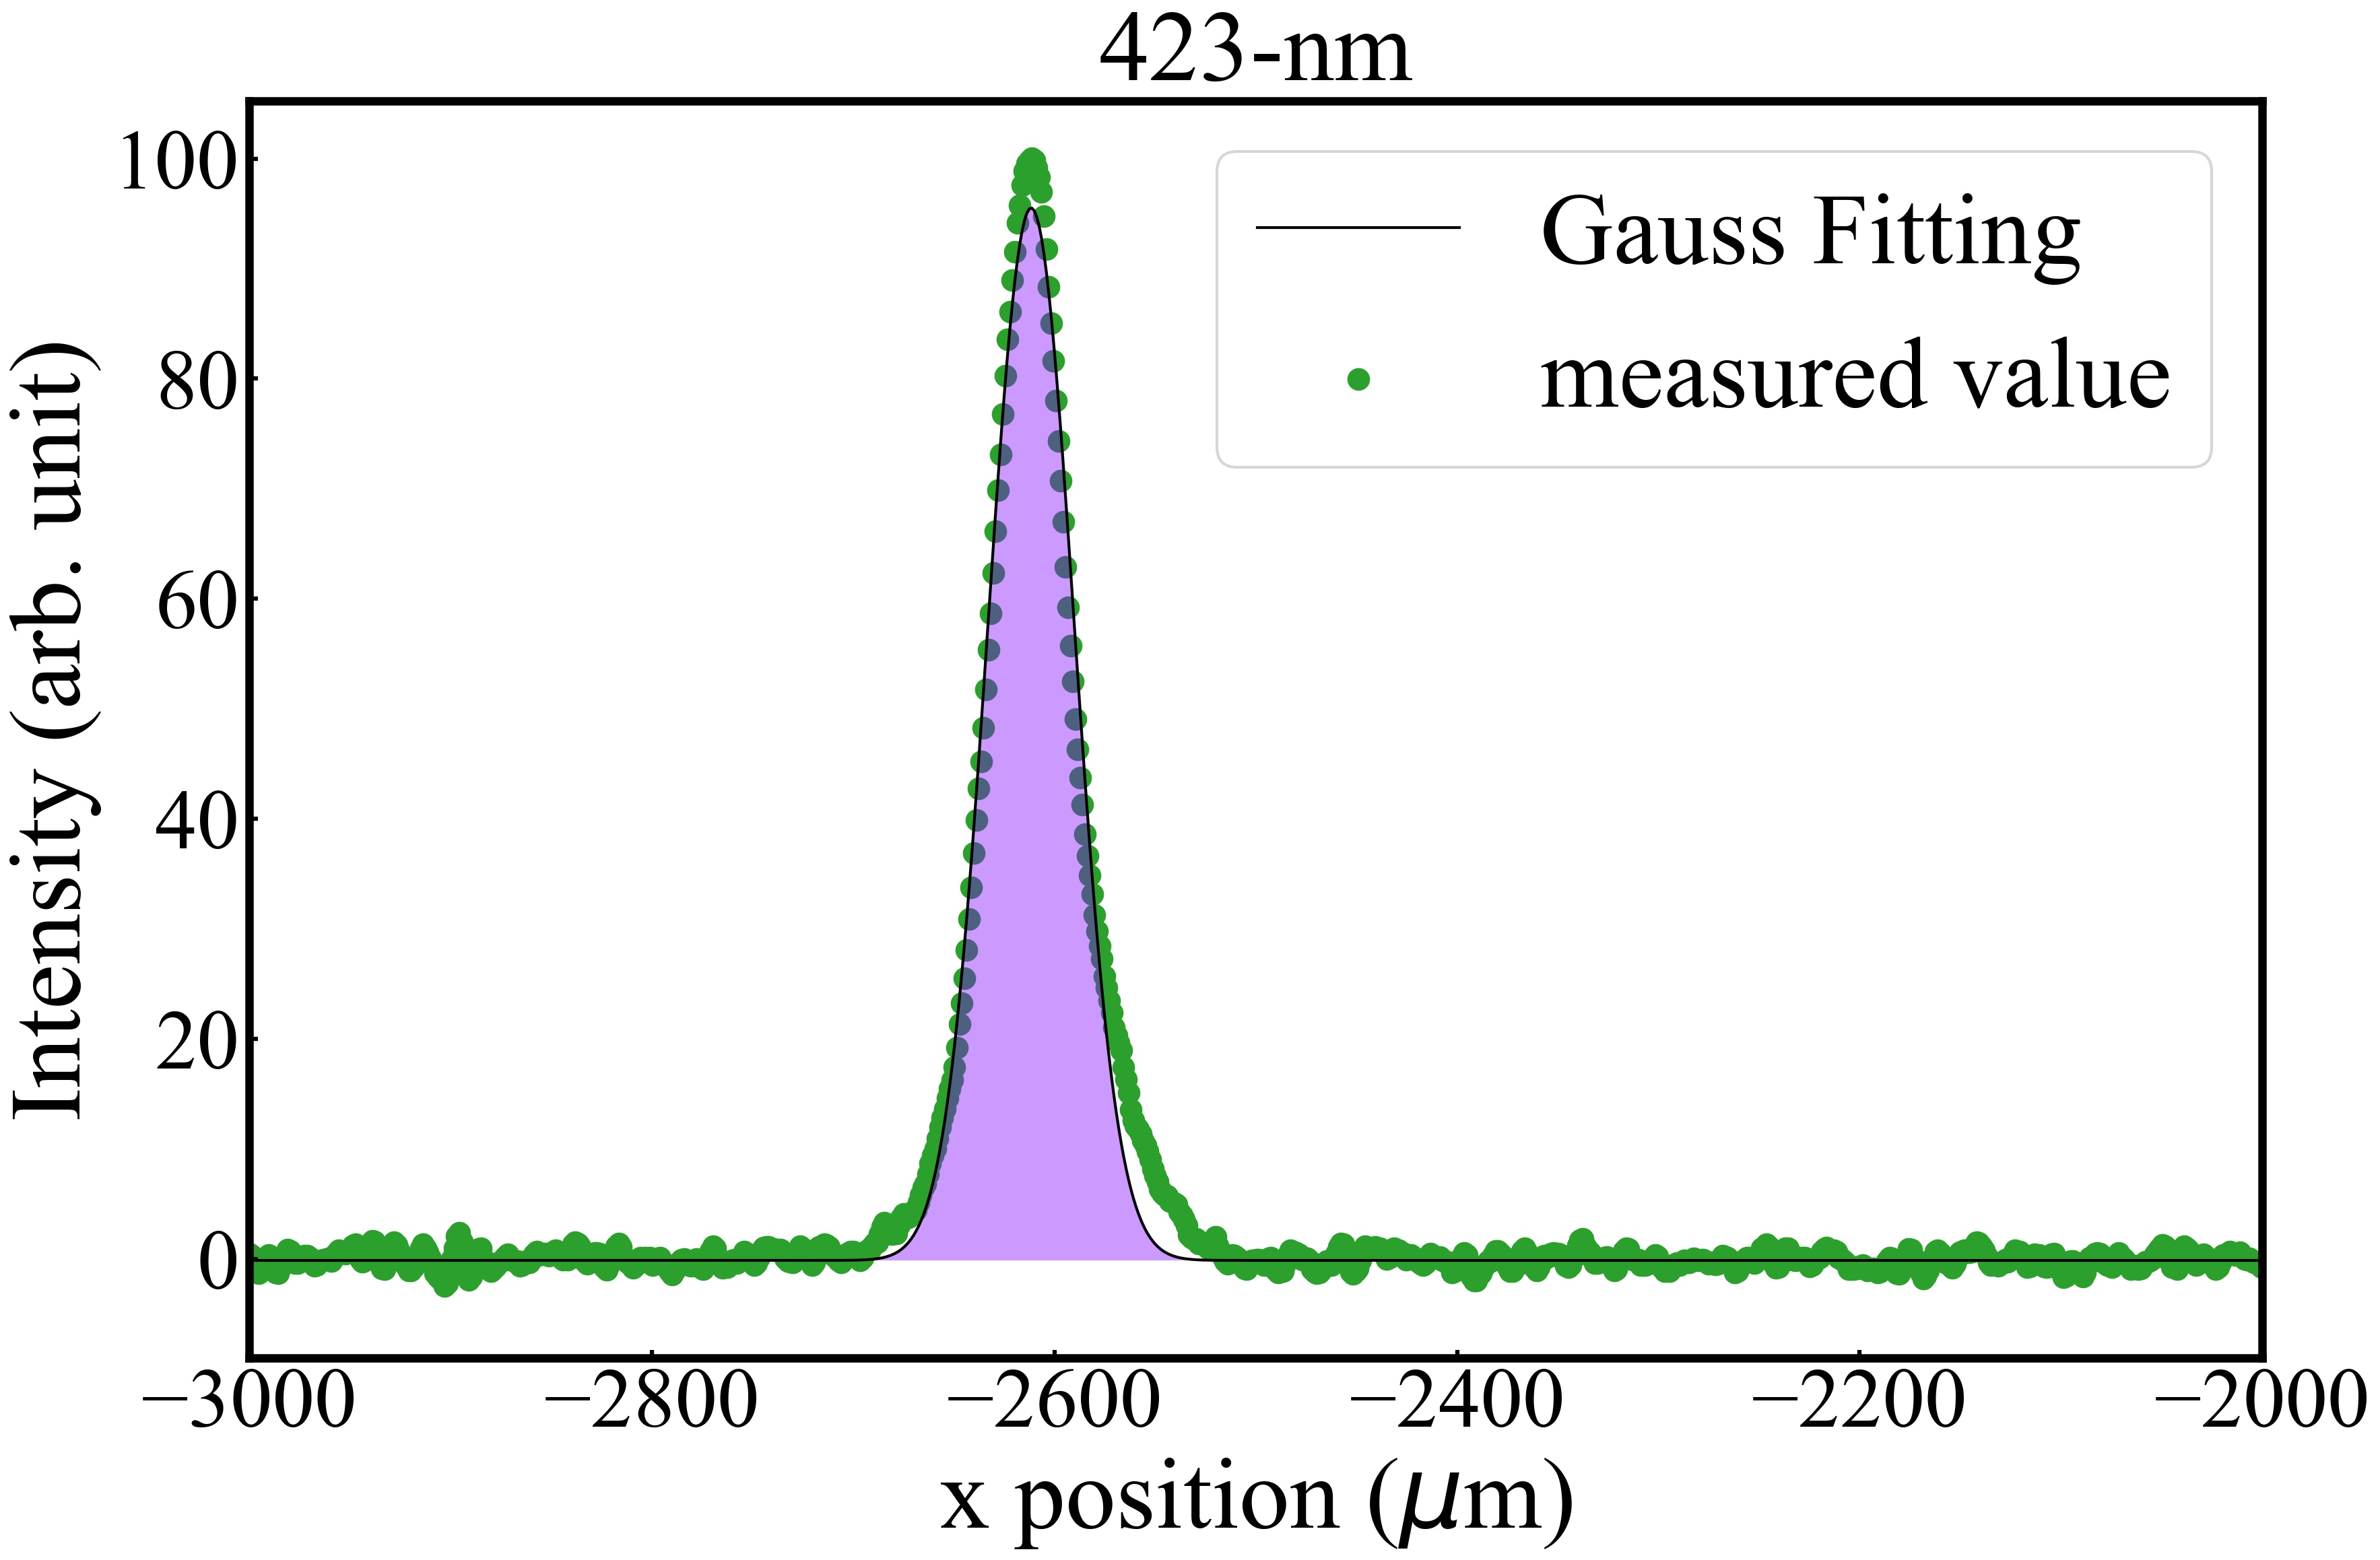
\includegraphics[width = 0.98\columnwidth]{./experimental_setup/figure/423GaussianFittingXpos.jpg}
	\end{center}
	\end{minipage}
	\begin{minipage}{0.48\linewidth}
	\begin{center}
		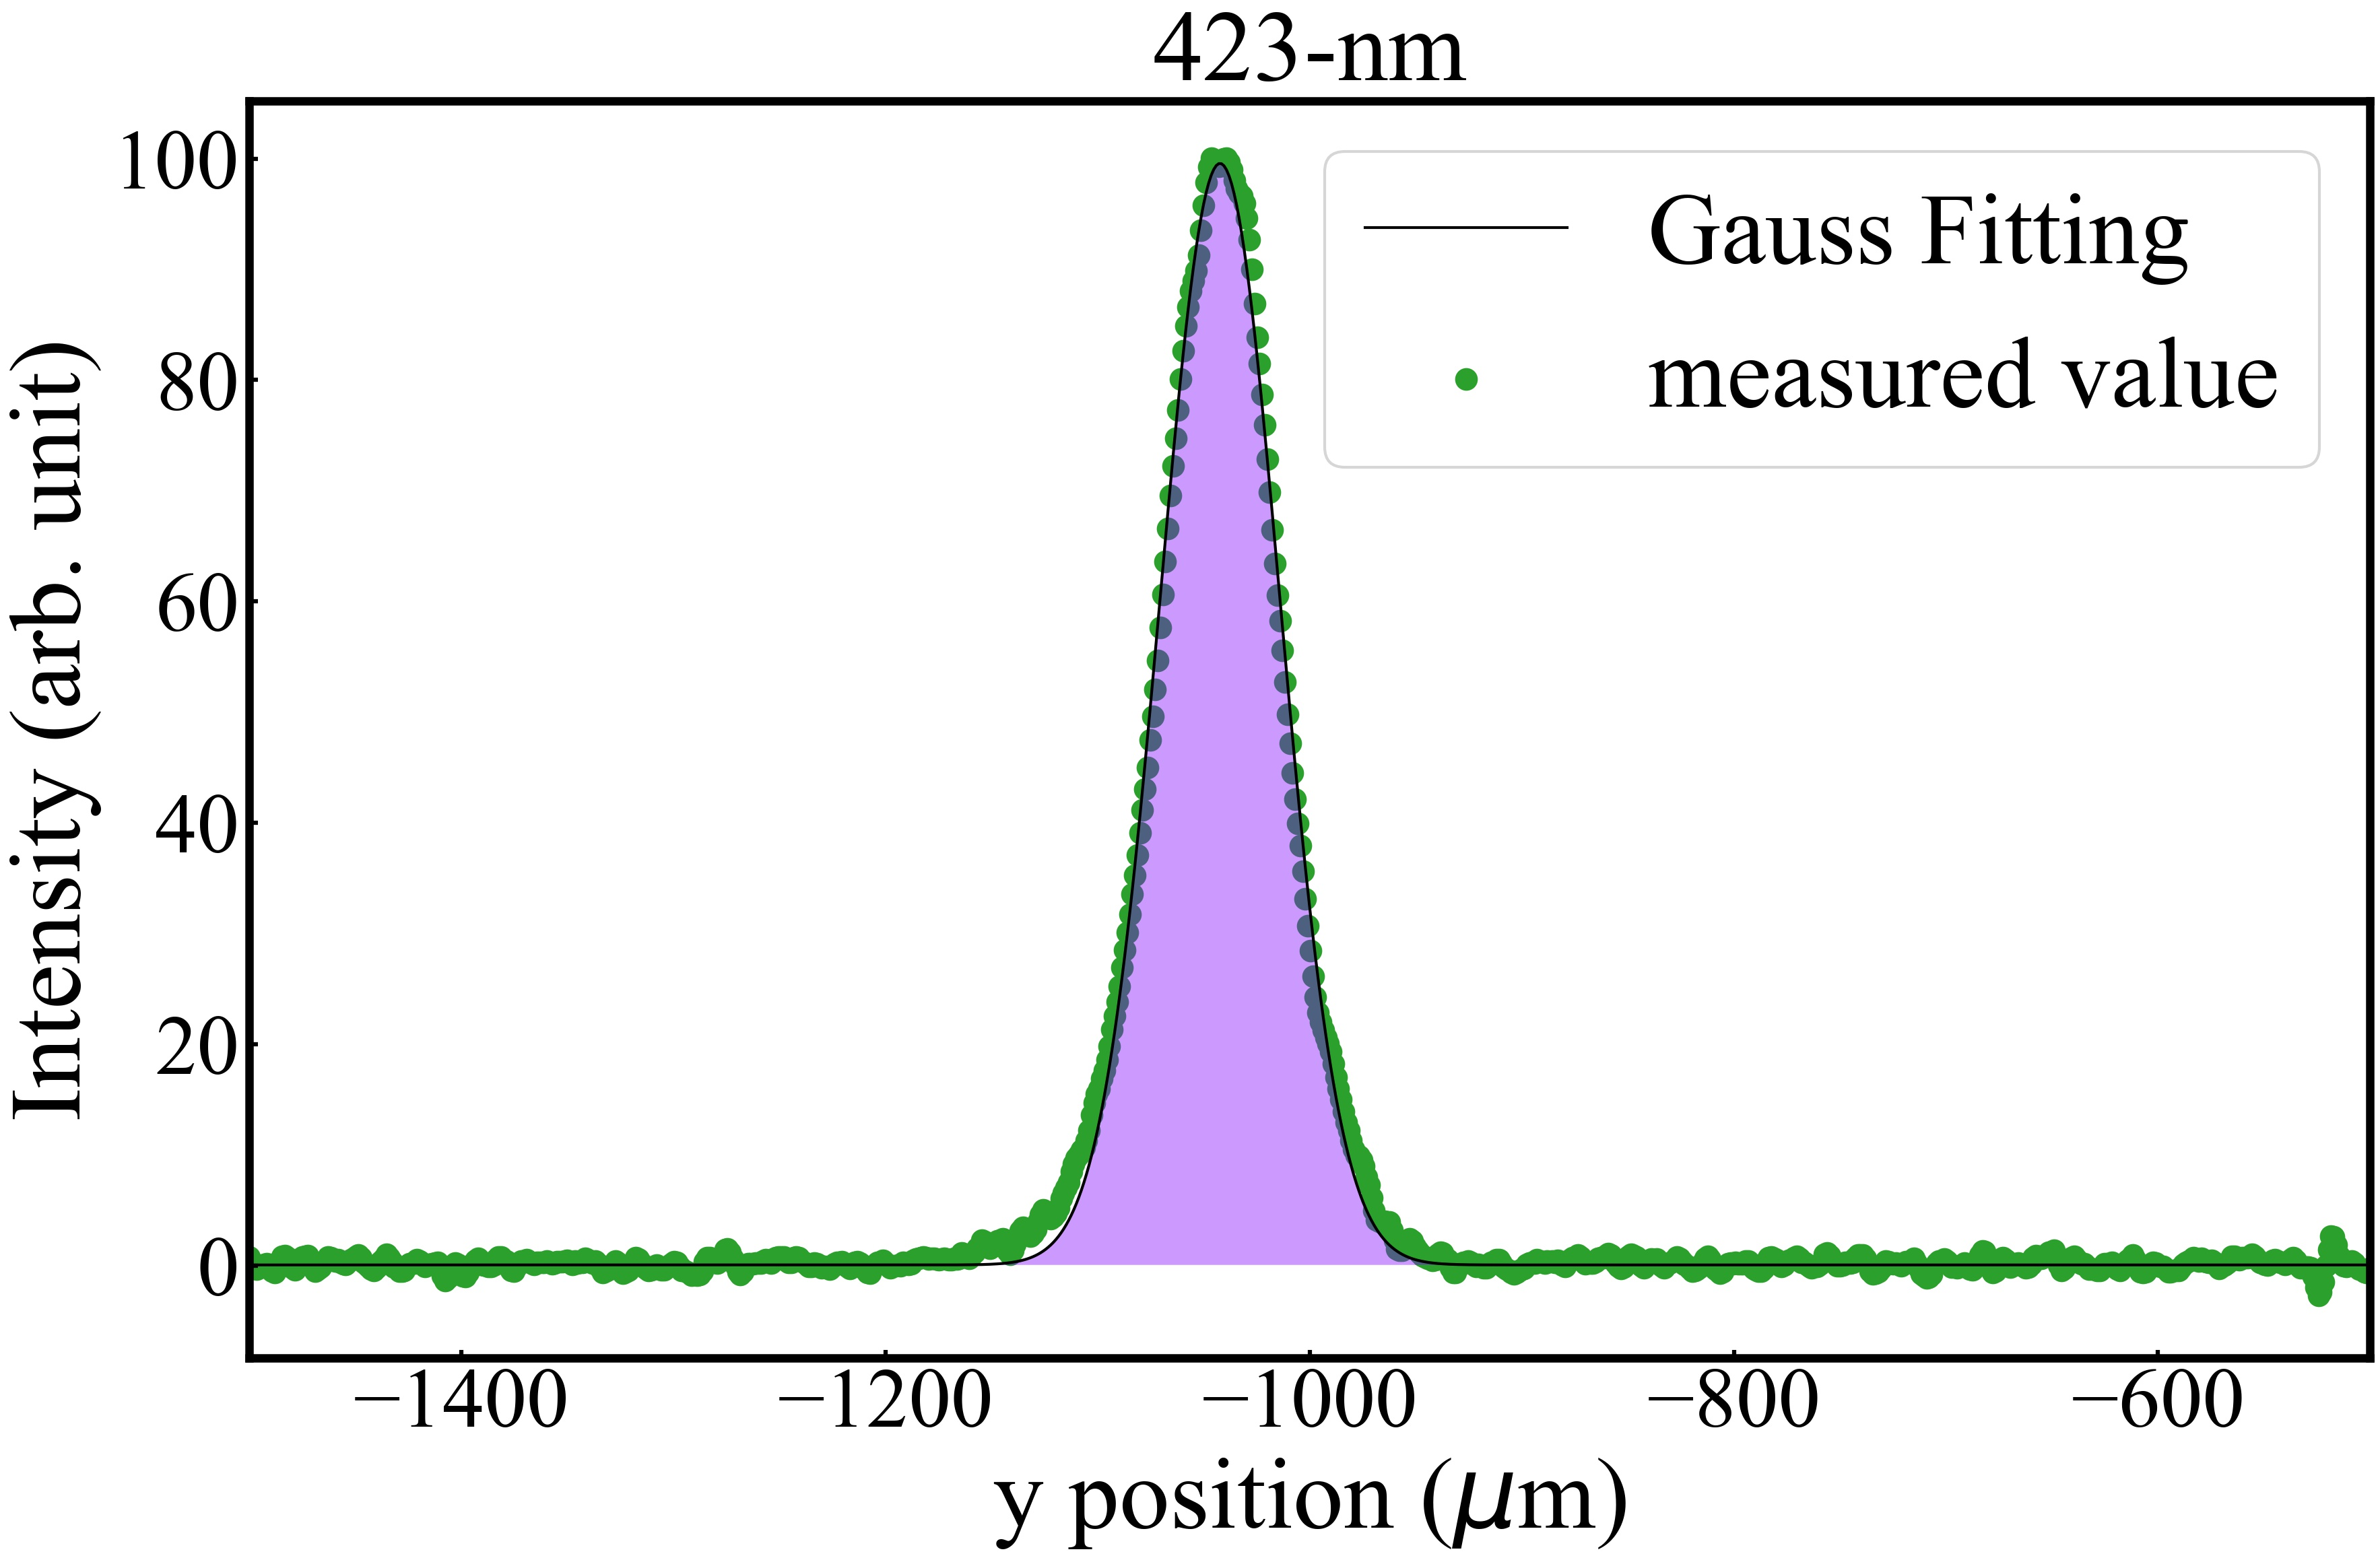
\includegraphics[width=0.98\columnwidth]{./experimental_setup/figure/423GaussianFittingYpos.jpg}
	\end{center}
	\end{minipage}
	%%%78
	\begin{minipage}{0.48\linewidth}
	\begin{center}
		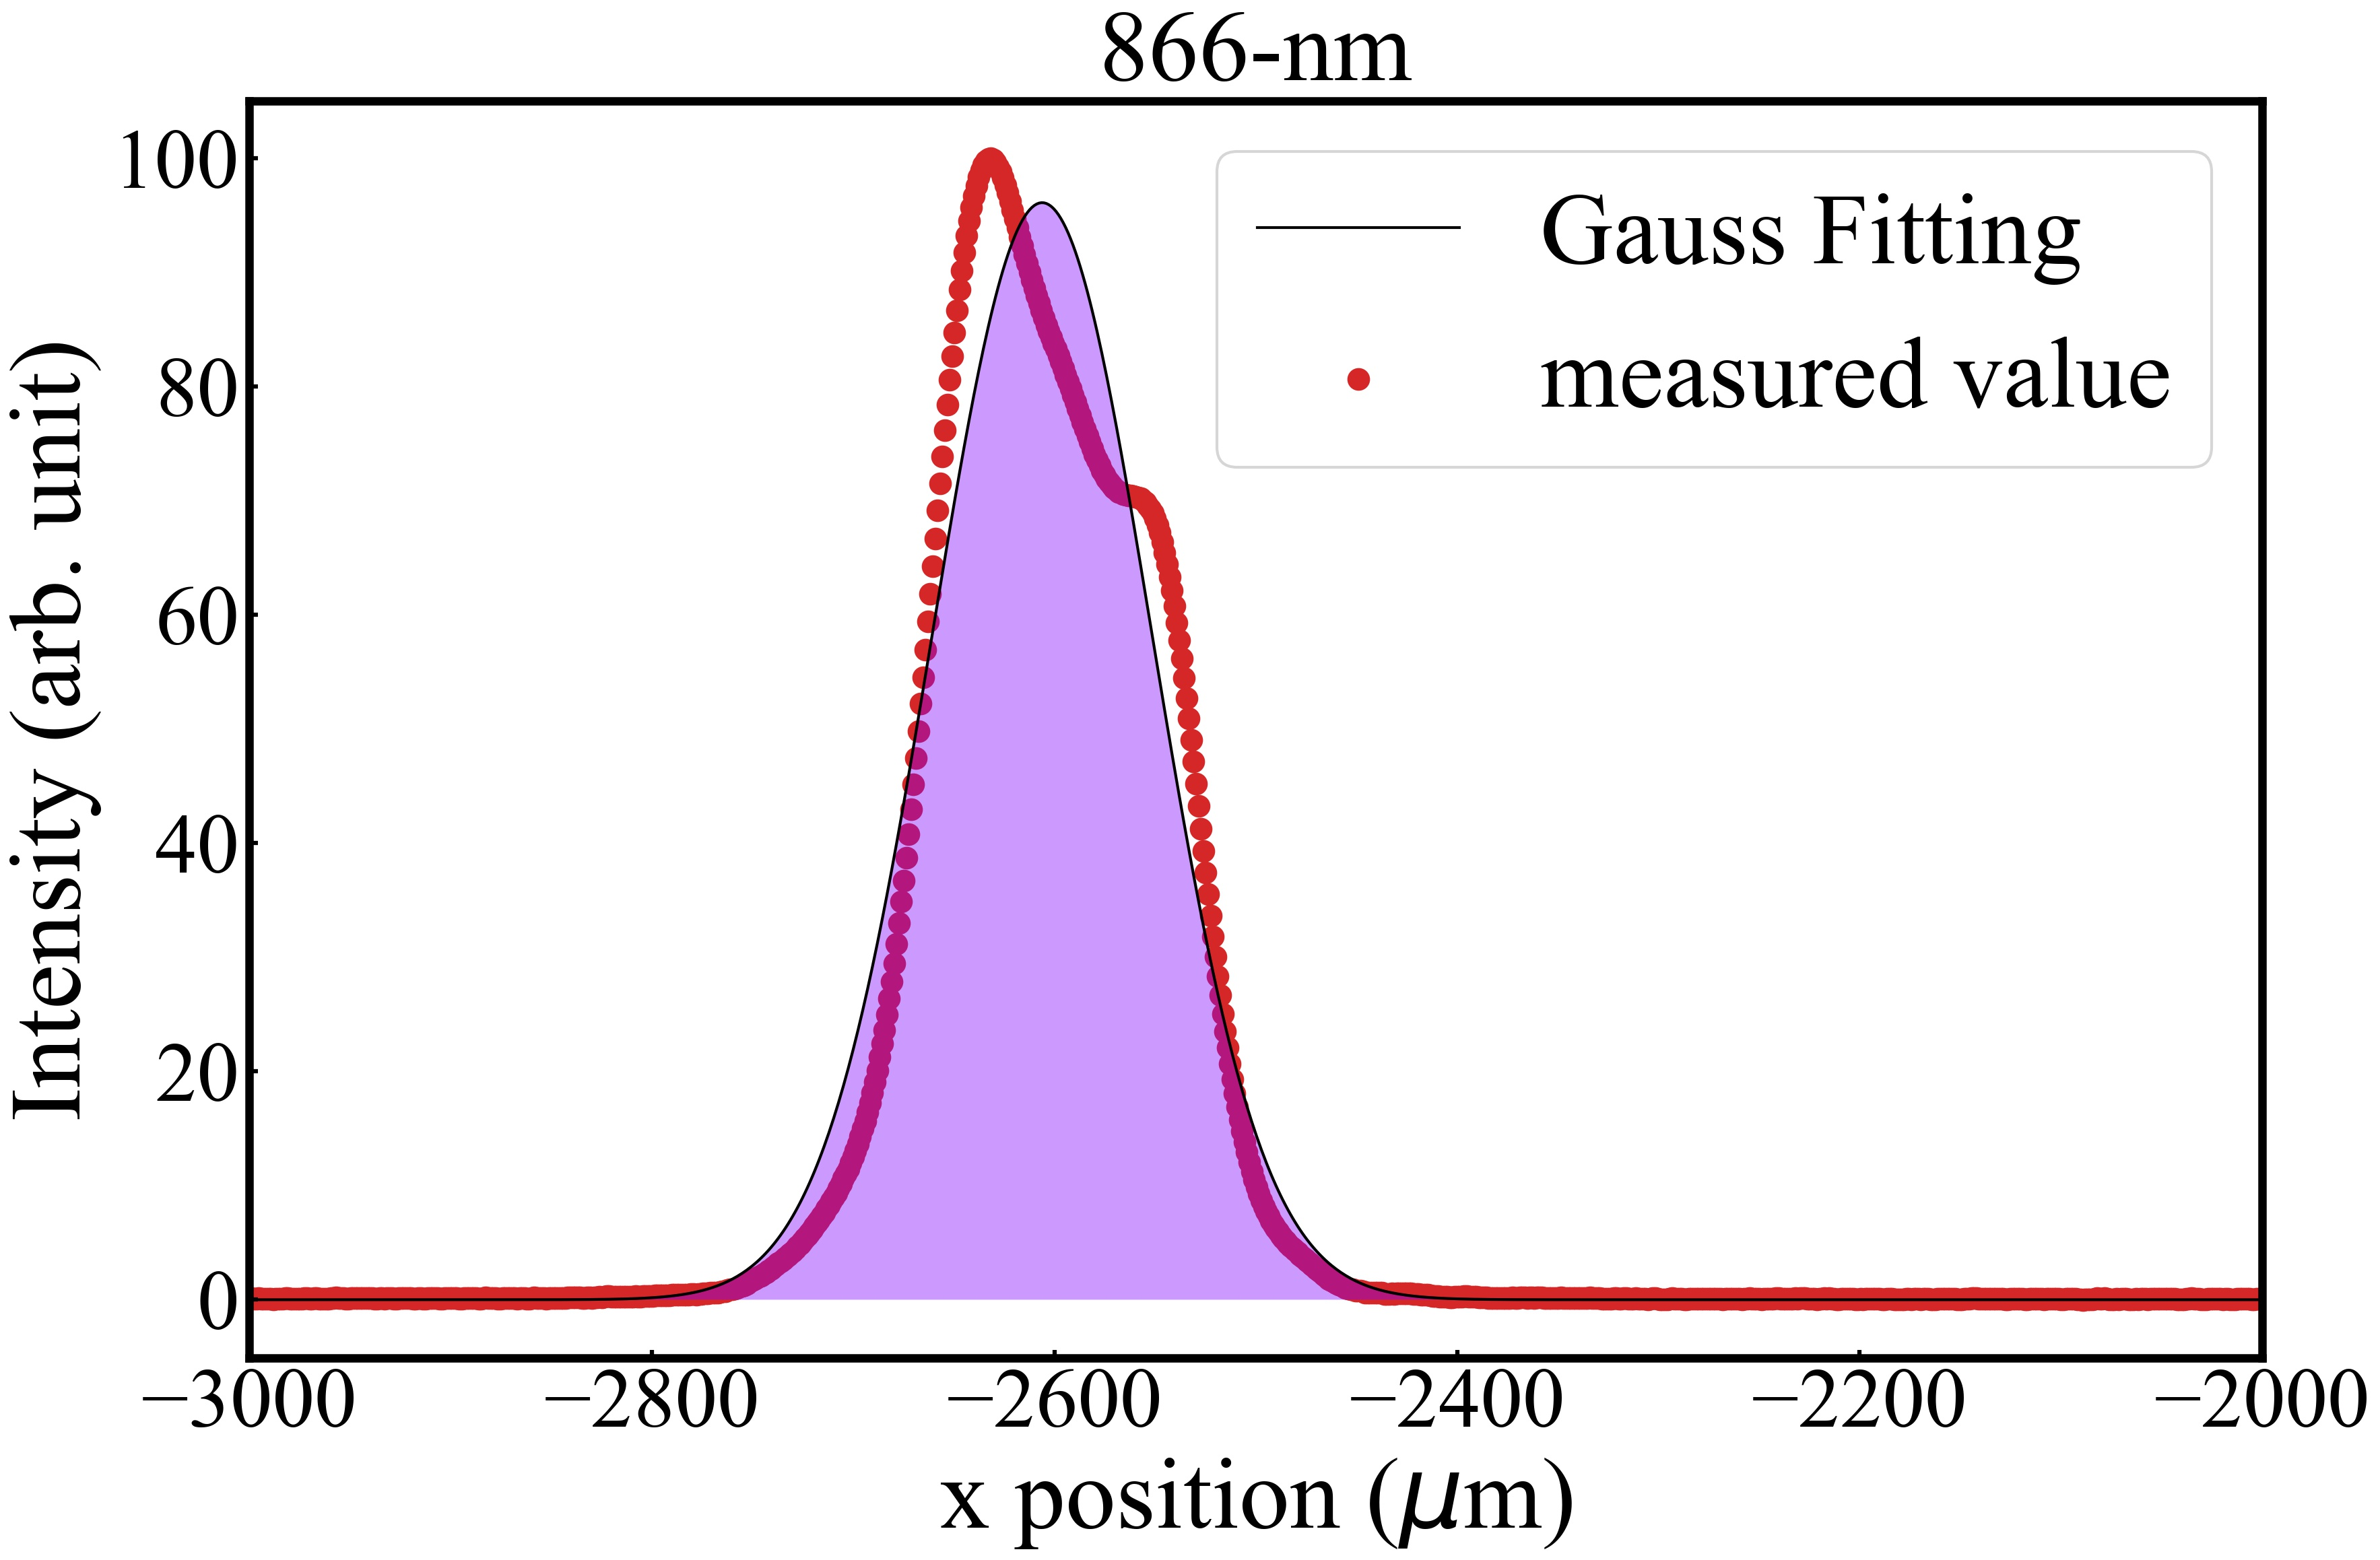
\includegraphics[width = 0.98\columnwidth]{./experimental_setup/figure/866GaussianFittingXpos.jpg}
	\end{center}
	\end{minipage}
	\begin{minipage}{0.48\linewidth}
	\begin{center}
		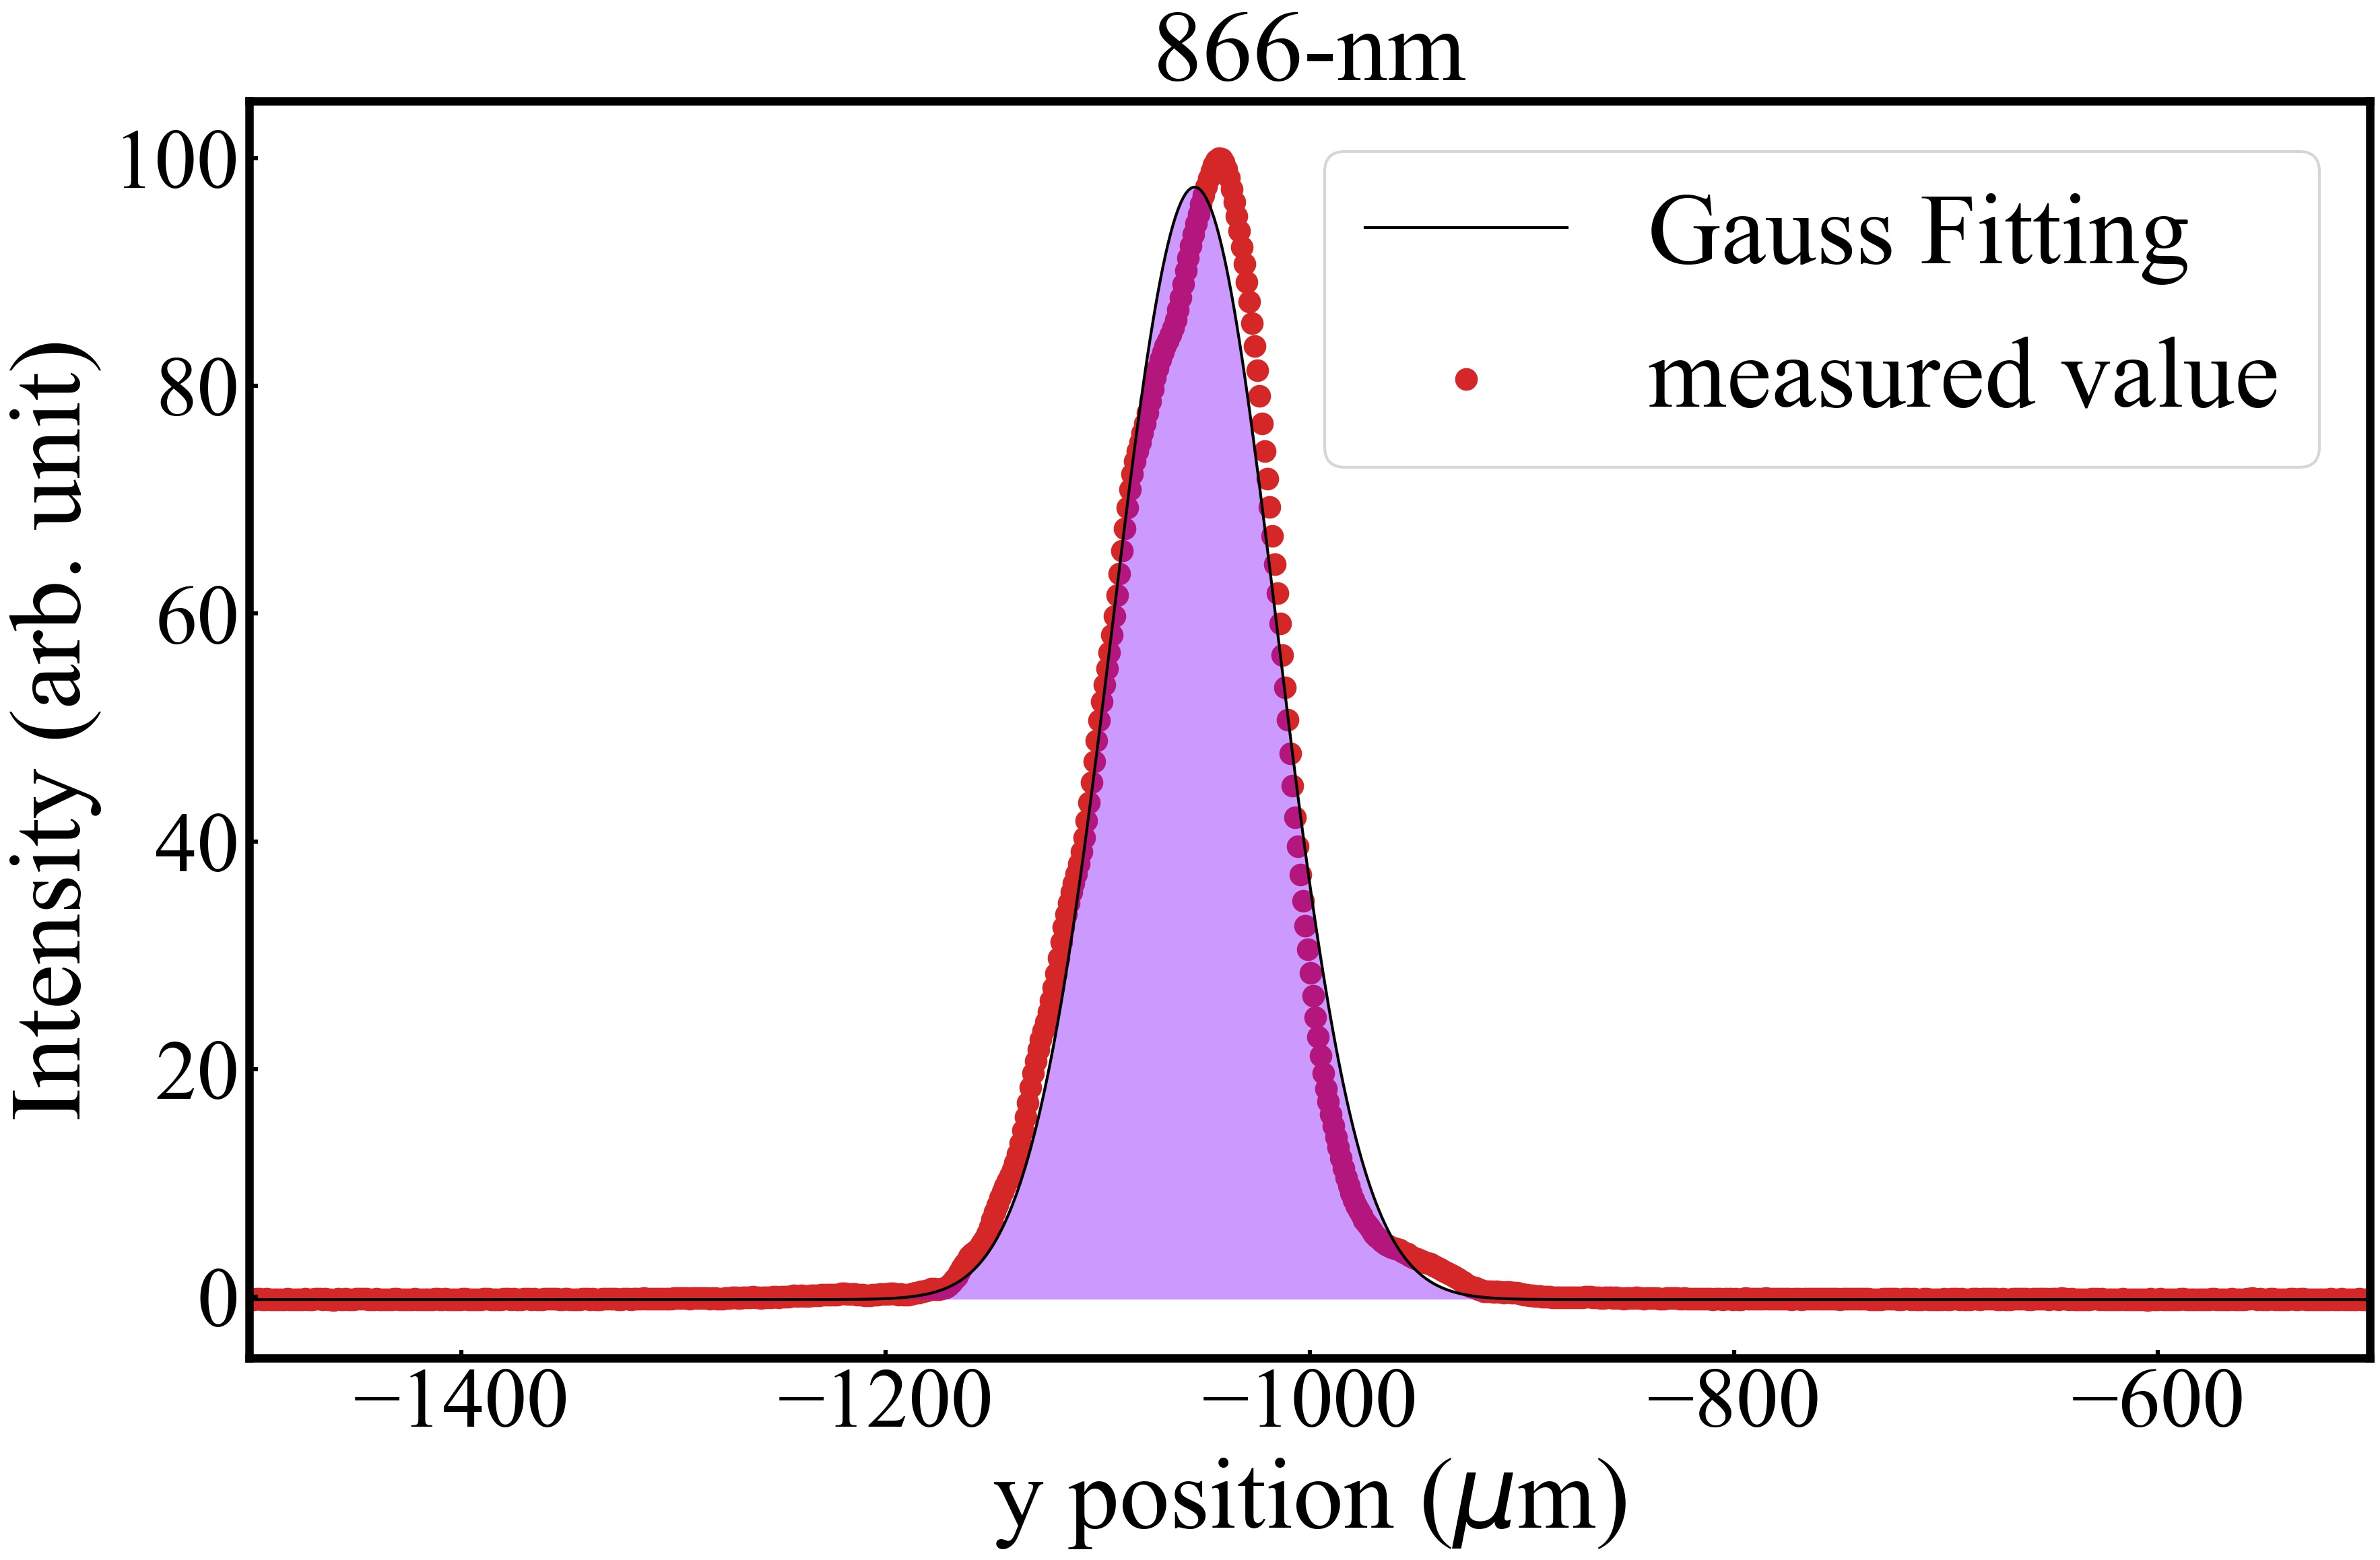
\includegraphics[width = 0.98\columnwidth]{./experimental_setup/figure/866GaussianFittingYpos.jpg}
	\end{center}
	\end{minipage}
	\caption{各波長に対してx,y方向それぞれのビームプロファイルにガウシアンフィッティングをかけた結果}
	\label{fig:GaussianFitting}
	\end{center}
\end{figure}
%
\clearpage
%
\section{検出系}
\Fig{Detect}ににイオンの捕獲を行うために必要な実験装置を示す.dc電圧の印加はLabViewを用いて行う.PC1で電圧値の設定を行いDAQへ信号を送る.信号を受け取ったDAQから指定されたdc電圧が出力されLPFを介してプレーナートラップへ印加される.rf電圧の印加には発振器を用いる.CH1から出力されるrf電圧はrf電極に印加され,CH2から出力されるrf電圧はcenter-rf電極に印加される.そして,プレーナートラップの電極表面に垂直な方向からイオンの蛍光をImage Intensifier(I. I. )と汎用CCDカメラを用いて集光を行い,PC2で画像を表示させている.

\begin{figure}[h]
	\begin{center}
		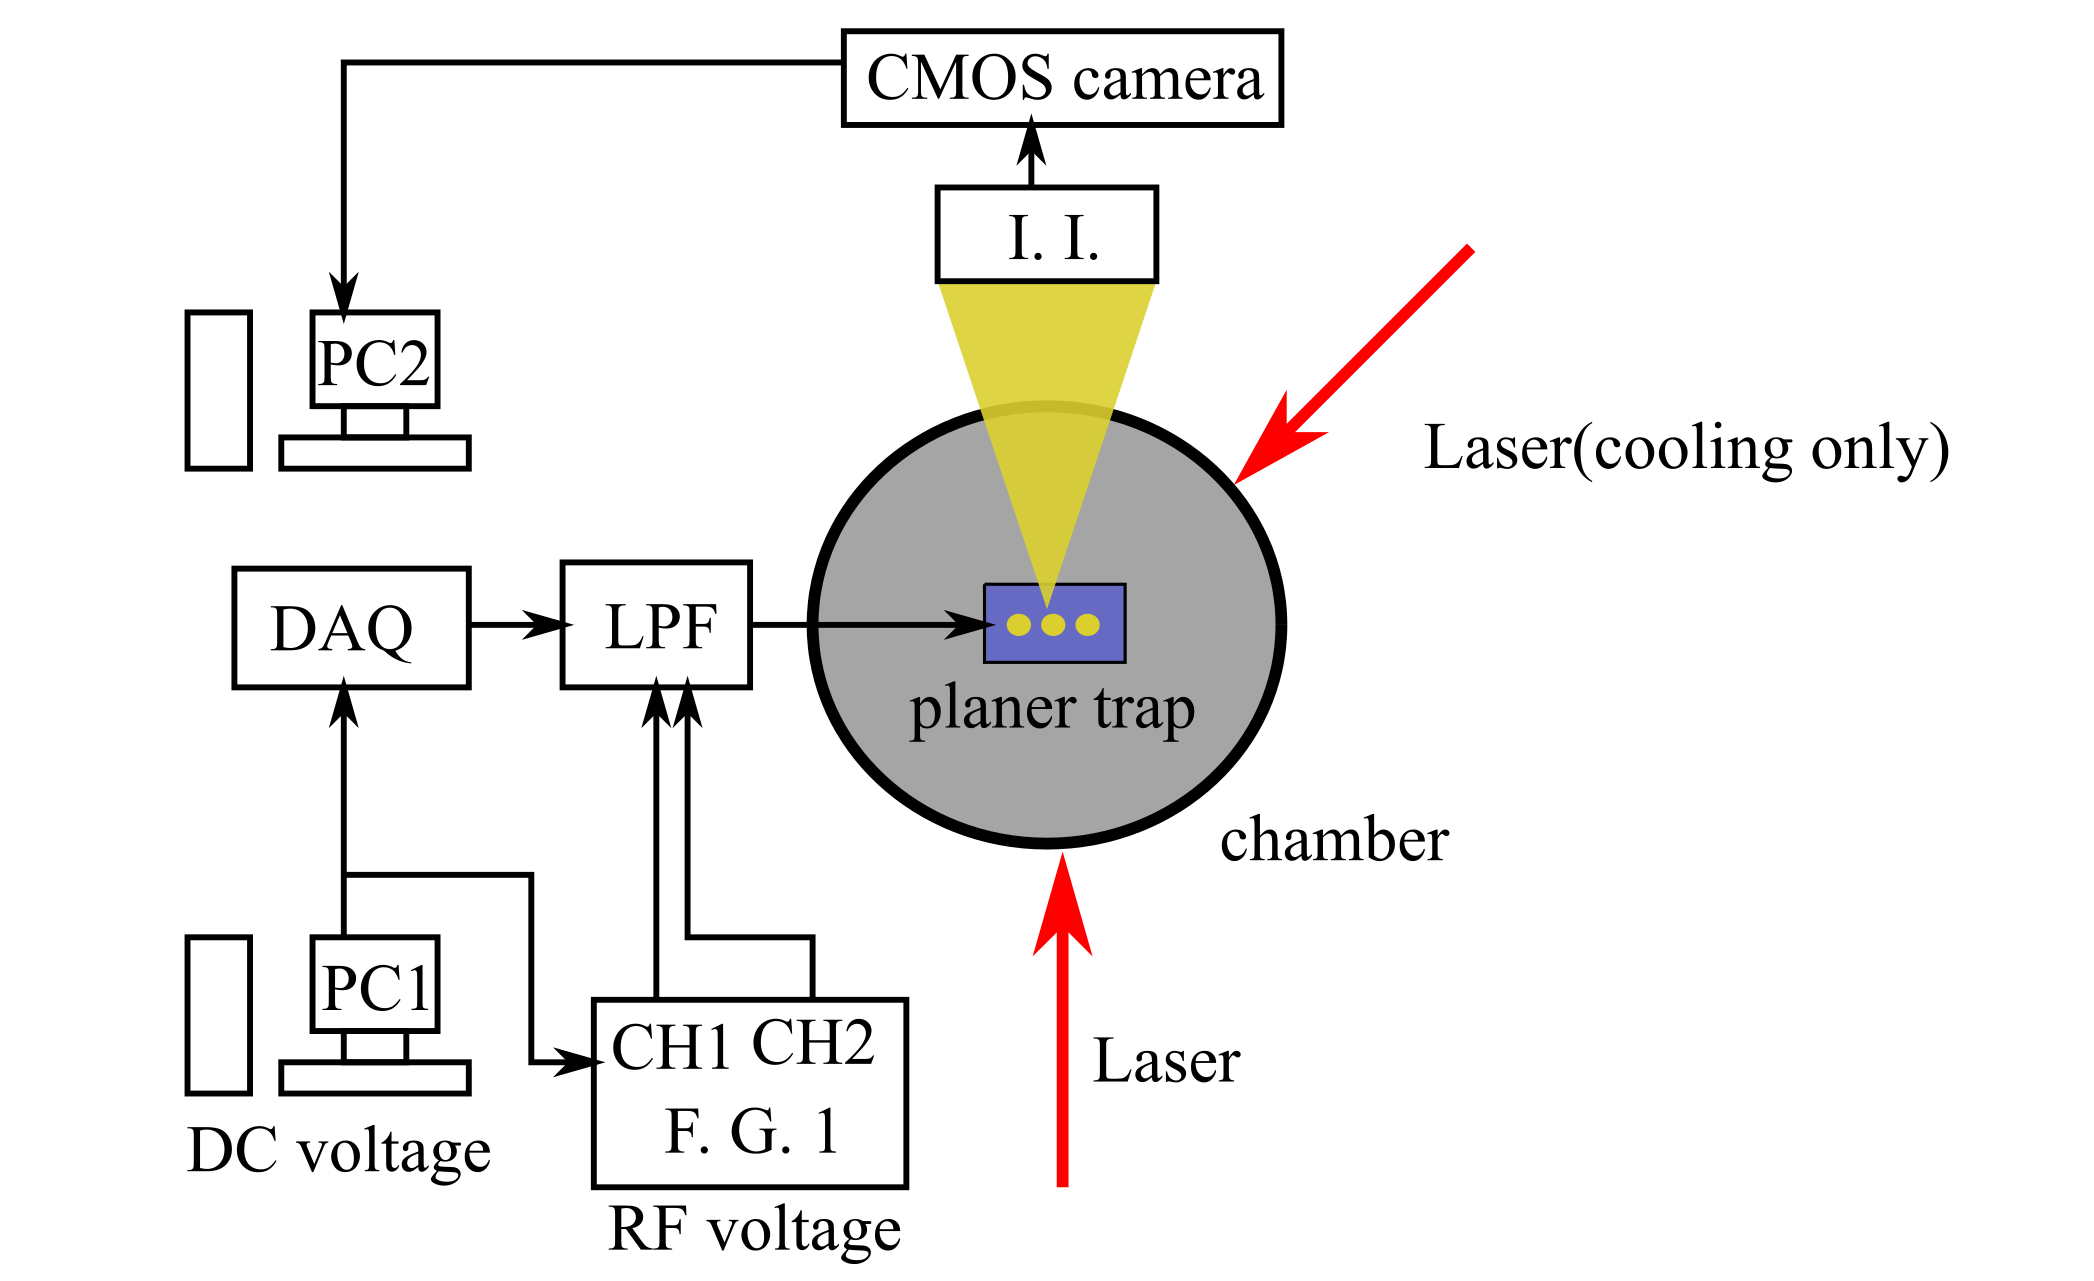
\includegraphics[width = 0.6\linewidth]{./experimental_setup/figure/Detect.png}
		\caption{実験装置(LPF : Low Pass Filter,DAQ : Data AcQusition,I.I. : Image Intensifier,F.G. Function Generator)}
		\label{fig:Detect}
	\end{center}
\end{figure}